% Options for packages loaded elsewhere
\PassOptionsToPackage{unicode}{hyperref}
\PassOptionsToPackage{hyphens}{url}
\PassOptionsToPackage{dvipsnames,svgnames,x11names}{xcolor}
%
\documentclass[
  letterpaper,
  DIV=11,
  numbers=noendperiod]{scrreprt}

\usepackage{amsmath,amssymb}
\usepackage{lmodern}
\usepackage{iftex}
\ifPDFTeX
  \usepackage[T1]{fontenc}
  \usepackage[utf8]{inputenc}
  \usepackage{textcomp} % provide euro and other symbols
\else % if luatex or xetex
  \usepackage{unicode-math}
  \defaultfontfeatures{Scale=MatchLowercase}
  \defaultfontfeatures[\rmfamily]{Ligatures=TeX,Scale=1}
\fi
% Use upquote if available, for straight quotes in verbatim environments
\IfFileExists{upquote.sty}{\usepackage{upquote}}{}
\IfFileExists{microtype.sty}{% use microtype if available
  \usepackage[]{microtype}
  \UseMicrotypeSet[protrusion]{basicmath} % disable protrusion for tt fonts
}{}
\makeatletter
\@ifundefined{KOMAClassName}{% if non-KOMA class
  \IfFileExists{parskip.sty}{%
    \usepackage{parskip}
  }{% else
    \setlength{\parindent}{0pt}
    \setlength{\parskip}{6pt plus 2pt minus 1pt}}
}{% if KOMA class
  \KOMAoptions{parskip=half}}
\makeatother
\usepackage{xcolor}
\setlength{\emergencystretch}{3em} % prevent overfull lines
\setcounter{secnumdepth}{5}
% Make \paragraph and \subparagraph free-standing
\ifx\paragraph\undefined\else
  \let\oldparagraph\paragraph
  \renewcommand{\paragraph}[1]{\oldparagraph{#1}\mbox{}}
\fi
\ifx\subparagraph\undefined\else
  \let\oldsubparagraph\subparagraph
  \renewcommand{\subparagraph}[1]{\oldsubparagraph{#1}\mbox{}}
\fi

\usepackage{color}
\usepackage{fancyvrb}
\newcommand{\VerbBar}{|}
\newcommand{\VERB}{\Verb[commandchars=\\\{\}]}
\DefineVerbatimEnvironment{Highlighting}{Verbatim}{commandchars=\\\{\}}
% Add ',fontsize=\small' for more characters per line
\usepackage{framed}
\definecolor{shadecolor}{RGB}{241,243,245}
\newenvironment{Shaded}{\begin{snugshade}}{\end{snugshade}}
\newcommand{\AlertTok}[1]{\textcolor[rgb]{0.68,0.00,0.00}{#1}}
\newcommand{\AnnotationTok}[1]{\textcolor[rgb]{0.37,0.37,0.37}{#1}}
\newcommand{\AttributeTok}[1]{\textcolor[rgb]{0.40,0.45,0.13}{#1}}
\newcommand{\BaseNTok}[1]{\textcolor[rgb]{0.68,0.00,0.00}{#1}}
\newcommand{\BuiltInTok}[1]{\textcolor[rgb]{0.00,0.23,0.31}{#1}}
\newcommand{\CharTok}[1]{\textcolor[rgb]{0.13,0.47,0.30}{#1}}
\newcommand{\CommentTok}[1]{\textcolor[rgb]{0.37,0.37,0.37}{#1}}
\newcommand{\CommentVarTok}[1]{\textcolor[rgb]{0.37,0.37,0.37}{\textit{#1}}}
\newcommand{\ConstantTok}[1]{\textcolor[rgb]{0.56,0.35,0.01}{#1}}
\newcommand{\ControlFlowTok}[1]{\textcolor[rgb]{0.00,0.23,0.31}{#1}}
\newcommand{\DataTypeTok}[1]{\textcolor[rgb]{0.68,0.00,0.00}{#1}}
\newcommand{\DecValTok}[1]{\textcolor[rgb]{0.68,0.00,0.00}{#1}}
\newcommand{\DocumentationTok}[1]{\textcolor[rgb]{0.37,0.37,0.37}{\textit{#1}}}
\newcommand{\ErrorTok}[1]{\textcolor[rgb]{0.68,0.00,0.00}{#1}}
\newcommand{\ExtensionTok}[1]{\textcolor[rgb]{0.00,0.23,0.31}{#1}}
\newcommand{\FloatTok}[1]{\textcolor[rgb]{0.68,0.00,0.00}{#1}}
\newcommand{\FunctionTok}[1]{\textcolor[rgb]{0.28,0.35,0.67}{#1}}
\newcommand{\ImportTok}[1]{\textcolor[rgb]{0.00,0.46,0.62}{#1}}
\newcommand{\InformationTok}[1]{\textcolor[rgb]{0.37,0.37,0.37}{#1}}
\newcommand{\KeywordTok}[1]{\textcolor[rgb]{0.00,0.23,0.31}{#1}}
\newcommand{\NormalTok}[1]{\textcolor[rgb]{0.00,0.23,0.31}{#1}}
\newcommand{\OperatorTok}[1]{\textcolor[rgb]{0.37,0.37,0.37}{#1}}
\newcommand{\OtherTok}[1]{\textcolor[rgb]{0.00,0.23,0.31}{#1}}
\newcommand{\PreprocessorTok}[1]{\textcolor[rgb]{0.68,0.00,0.00}{#1}}
\newcommand{\RegionMarkerTok}[1]{\textcolor[rgb]{0.00,0.23,0.31}{#1}}
\newcommand{\SpecialCharTok}[1]{\textcolor[rgb]{0.37,0.37,0.37}{#1}}
\newcommand{\SpecialStringTok}[1]{\textcolor[rgb]{0.13,0.47,0.30}{#1}}
\newcommand{\StringTok}[1]{\textcolor[rgb]{0.13,0.47,0.30}{#1}}
\newcommand{\VariableTok}[1]{\textcolor[rgb]{0.07,0.07,0.07}{#1}}
\newcommand{\VerbatimStringTok}[1]{\textcolor[rgb]{0.13,0.47,0.30}{#1}}
\newcommand{\WarningTok}[1]{\textcolor[rgb]{0.37,0.37,0.37}{\textit{#1}}}

\providecommand{\tightlist}{%
  \setlength{\itemsep}{0pt}\setlength{\parskip}{0pt}}\usepackage{longtable,booktabs,array}
\usepackage{calc} % for calculating minipage widths
% Correct order of tables after \paragraph or \subparagraph
\usepackage{etoolbox}
\makeatletter
\patchcmd\longtable{\par}{\if@noskipsec\mbox{}\fi\par}{}{}
\makeatother
% Allow footnotes in longtable head/foot
\IfFileExists{footnotehyper.sty}{\usepackage{footnotehyper}}{\usepackage{footnote}}
\makesavenoteenv{longtable}
\usepackage{graphicx}
\makeatletter
\def\maxwidth{\ifdim\Gin@nat@width>\linewidth\linewidth\else\Gin@nat@width\fi}
\def\maxheight{\ifdim\Gin@nat@height>\textheight\textheight\else\Gin@nat@height\fi}
\makeatother
% Scale images if necessary, so that they will not overflow the page
% margins by default, and it is still possible to overwrite the defaults
% using explicit options in \includegraphics[width, height, ...]{}
\setkeys{Gin}{width=\maxwidth,height=\maxheight,keepaspectratio}
% Set default figure placement to htbp
\makeatletter
\def\fps@figure{htbp}
\makeatother
\newlength{\cslhangindent}
\setlength{\cslhangindent}{1.5em}
\newlength{\csllabelwidth}
\setlength{\csllabelwidth}{3em}
\newlength{\cslentryspacingunit} % times entry-spacing
\setlength{\cslentryspacingunit}{\parskip}
\newenvironment{CSLReferences}[2] % #1 hanging-ident, #2 entry spacing
 {% don't indent paragraphs
  \setlength{\parindent}{0pt}
  % turn on hanging indent if param 1 is 1
  \ifodd #1
  \let\oldpar\par
  \def\par{\hangindent=\cslhangindent\oldpar}
  \fi
  % set entry spacing
  \setlength{\parskip}{#2\cslentryspacingunit}
 }%
 {}
\usepackage{calc}
\newcommand{\CSLBlock}[1]{#1\hfill\break}
\newcommand{\CSLLeftMargin}[1]{\parbox[t]{\csllabelwidth}{#1}}
\newcommand{\CSLRightInline}[1]{\parbox[t]{\linewidth - \csllabelwidth}{#1}\break}
\newcommand{\CSLIndent}[1]{\hspace{\cslhangindent}#1}

\KOMAoption{captions}{tableheading}
\makeatletter
\@ifpackageloaded{tcolorbox}{}{\usepackage[many]{tcolorbox}}
\@ifpackageloaded{fontawesome5}{}{\usepackage{fontawesome5}}
\definecolor{quarto-callout-color}{HTML}{909090}
\definecolor{quarto-callout-note-color}{HTML}{0758E5}
\definecolor{quarto-callout-important-color}{HTML}{CC1914}
\definecolor{quarto-callout-warning-color}{HTML}{EB9113}
\definecolor{quarto-callout-tip-color}{HTML}{00A047}
\definecolor{quarto-callout-caution-color}{HTML}{FC5300}
\definecolor{quarto-callout-color-frame}{HTML}{acacac}
\definecolor{quarto-callout-note-color-frame}{HTML}{4582ec}
\definecolor{quarto-callout-important-color-frame}{HTML}{d9534f}
\definecolor{quarto-callout-warning-color-frame}{HTML}{f0ad4e}
\definecolor{quarto-callout-tip-color-frame}{HTML}{02b875}
\definecolor{quarto-callout-caution-color-frame}{HTML}{fd7e14}
\makeatother
\makeatletter
\makeatother
\makeatletter
\@ifpackageloaded{bookmark}{}{\usepackage{bookmark}}
\makeatother
\makeatletter
\@ifpackageloaded{caption}{}{\usepackage{caption}}
\AtBeginDocument{%
\ifdefined\contentsname
  \renewcommand*\contentsname{Table of contents}
\else
  \newcommand\contentsname{Table of contents}
\fi
\ifdefined\listfigurename
  \renewcommand*\listfigurename{List of Figures}
\else
  \newcommand\listfigurename{List of Figures}
\fi
\ifdefined\listtablename
  \renewcommand*\listtablename{List of Tables}
\else
  \newcommand\listtablename{List of Tables}
\fi
\ifdefined\figurename
  \renewcommand*\figurename{Figure}
\else
  \newcommand\figurename{Figure}
\fi
\ifdefined\tablename
  \renewcommand*\tablename{Table}
\else
  \newcommand\tablename{Table}
\fi
}
\@ifpackageloaded{float}{}{\usepackage{float}}
\floatstyle{ruled}
\@ifundefined{c@chapter}{\newfloat{codelisting}{h}{lop}}{\newfloat{codelisting}{h}{lop}[chapter]}
\floatname{codelisting}{Listing}
\newcommand*\listoflistings{\listof{codelisting}{List of Listings}}
\makeatother
\makeatletter
\@ifpackageloaded{caption}{}{\usepackage{caption}}
\@ifpackageloaded{subcaption}{}{\usepackage{subcaption}}
\makeatother
\makeatletter
\@ifpackageloaded{tcolorbox}{}{\usepackage[many]{tcolorbox}}
\makeatother
\makeatletter
\@ifundefined{shadecolor}{\definecolor{shadecolor}{rgb}{.97, .97, .97}}
\makeatother
\makeatletter
\makeatother
\ifLuaTeX
  \usepackage{selnolig}  % disable illegal ligatures
\fi
\IfFileExists{bookmark.sty}{\usepackage{bookmark}}{\usepackage{hyperref}}
\IfFileExists{xurl.sty}{\usepackage{xurl}}{} % add URL line breaks if available
\urlstyle{same} % disable monospaced font for URLs
\hypersetup{
  pdftitle={A touch of R in robotics},
  pdfauthor={Eric and Ian},
  colorlinks=true,
  linkcolor={blue},
  filecolor={Maroon},
  citecolor={Blue},
  urlcolor={Blue},
  pdfcreator={LaTeX via pandoc}}

\title{A touch of R in robotics}
\author{Eric and Ian}
\date{}

\begin{document}
\maketitle
\ifdefined\Shaded\renewenvironment{Shaded}{\begin{tcolorbox}[breakable, borderline west={3pt}{0pt}{shadecolor}, interior hidden, enhanced, sharp corners, boxrule=0pt, frame hidden]}{\end{tcolorbox}}\fi

\renewcommand*\contentsname{Table of contents}
{
\hypersetup{linkcolor=}
\setcounter{tocdepth}{2}
\tableofcontents
}
\bookmarksetup{startatroot}

\hypertarget{preface}{%
\chapter*{Preface}\label{preface}}
\addcontentsline{toc}{chapter}{Preface}

Hujambo and welcome to the accompanying guide for our
\href{https://www.rstudio.com/conference/}{rstudio::conf(2022)} talk:
\emph{\texttt{A\ Touch\ of\ R\ in\ Robotics}}.

In these series of notebooks, we try as much as possible to provide
detailed explanations of the methodologies used along with the
corresponding code.

We hope you enjoy it as much as we did 🤖.

\begin{tcolorbox}[enhanced jigsaw, colbacktitle=quarto-callout-note-color!10!white, opacityback=0, breakable, bottomtitle=1mm, coltitle=black, arc=.35mm, left=2mm, titlerule=0mm, rightrule=.15mm, title=\textcolor{quarto-callout-note-color}{\faInfo}\hspace{0.5em}{Note}, colframe=quarto-callout-note-color-frame, leftrule=.75mm, bottomrule=.15mm, toptitle=1mm, toprule=.15mm, opacitybacktitle=0.6, colback=white]
\texttt{Hujambo} is a \emph{Swahili} word used in the context of
\texttt{Hello} or \texttt{How\ are\ you?}. One typically replies with
\texttt{Sijambo} meaning \texttt{I\ am\ fine}
\end{tcolorbox}

combining R and Arduino to perform a pick and place action

\begin{figure}

{\centering \includegraphics[width=5.20833in,height=\textheight]{./images/comp_traj.mp4}

}

\end{figure}

\bookmarksetup{startatroot}

\hypertarget{speech-to-text}{%
\chapter{Speech to text}\label{speech-to-text}}

Ian Muchiri and Eric Wanjau

\hfill\break

This notebook contains a step by step guide on how to record audio in R
using the
\href{https://cran.r-project.org/web/packages/audio/audio.pdf}{audio
package} and convert the recording to text using Microsoft Azure
Cognitive Services, specifically the
\href{https://docs.microsoft.com/en-us/azure/cognitive-services/speech-service/rest-speech-to-text-short}{speech-to-text
service}.

I recently found myself working on a chess play automation project. The
user would issue a voice command describing the location of the piece
they want to move and their desired destination location, the data would
then processed and a chess move made. This was so cool and being the
R-nista that I am (i don't think this is a word, i have only come across
Pythonistas ) ,I thought to myself, maybe this can also be done in R and
voila, this article was born. For any feedback feel free to reach out at
\href{https://twitter.com/Entity_4004}{Ian}

\hypertarget{recording-audio-in-r-using-the-audio-package}{%
\section{Recording Audio in R using the audio
Package}\label{recording-audio-in-r-using-the-audio-package}}

We begin with the input which we plan to transcribe. In order to record
audio,we need to install and load the audio package

\begin{Shaded}
\begin{Highlighting}[]
\CommentTok{\#install the audio package}
\FunctionTok{install.packages}\NormalTok{(}\StringTok{"audio"}\NormalTok{)}
\end{Highlighting}
\end{Shaded}

We then proceed to setup the audio driver which we will use to record as
shown below:

\begin{Shaded}
\begin{Highlighting}[]
\CommentTok{\#Load the library}
\FunctionTok{library}\NormalTok{(audio)}
\CommentTok{\#Check which audio driver is set}
\FunctionTok{current.audio.driver}\NormalTok{()}
\end{Highlighting}
\end{Shaded}

\begin{Shaded}
\begin{Highlighting}[]
\CommentTok{\#if there is no driver set, view what drivers are available}
\FunctionTok{audio.drivers}\NormalTok{()}
\end{Highlighting}
\end{Shaded}

\begin{Shaded}
\begin{Highlighting}[]
\CommentTok{\#from the list provided, set which driver to use (default driver is always best)}
\FunctionTok{set.audio.driver}\NormalTok{(}\ConstantTok{NULL}\NormalTok{)}\CommentTok{\# sets the default audio driver}
\CommentTok{\#option 2}
\FunctionTok{set.audio.driver}\NormalTok{ (insert\_name\_here ) }\CommentTok{\#sets the audio driver to a driver other than the default}
\end{Highlighting}
\end{Shaded}

\begin{Shaded}
\begin{Highlighting}[]
\CommentTok{\#Checks and verifies that indeed the audio driver is set as per the command above}
\FunctionTok{current.audio.driver}\NormalTok{() }
\end{Highlighting}
\end{Shaded}

\hypertarget{recording-audio}{%
\subsection{Recording Audio}\label{recording-audio}}

Some of the key parameters in audio processing which we are going to
encounter during this exercise include:

\textbf{Sample rate:} This is the number of times per second a sound is
sampled and recorded.Therefore, if we use a sampling rate of say 8000
Hertz, a recording with a duration of 5 seconds will contain 40,000
samples (8000 * 5). The industry standard sampling rate commonly used is
44100 Hertz.

\textbf{Mono vs Stereo:} If you are a sound enthusiast, you've probably
come across these terms. Simply put, Mono sound is recorded and played
back using only \emph{one audio channel} e.g.~a guitarist recording
using one mic to pick up sound of the guitar and Stereo sound is
recorded and played through \emph{more than one channel.}

In our case we will use one audio channel(mono) and a sampling rate of
44100Hz. That being said let's start our recording

\begin{Shaded}
\begin{Highlighting}[]
\CommentTok{\#Set our recording time}
\NormalTok{rec\_time }\OtherTok{\textless{}{-}} \DecValTok{5} 

\CommentTok{\#Recording}
\NormalTok{Samples}\OtherTok{\textless{}{-}}\FunctionTok{rep}\NormalTok{(}\ConstantTok{NA\_real\_}\NormalTok{, }\DecValTok{44100} \SpecialCharTok{*}\NormalTok{ rec\_time) }\CommentTok{\#Defining number of samples recorded}
\FunctionTok{print}\NormalTok{(}\StringTok{"Start speaking"}\NormalTok{)}
\NormalTok{audio\_obj }\OtherTok{\textless{}{-}}\FunctionTok{record}\NormalTok{(Samples, }\DecValTok{44100}\NormalTok{, }\DecValTok{1}\NormalTok{) }\CommentTok{\#Create an audio instance with sample rate 44100 and mono channel}
\FunctionTok{wait}\NormalTok{(}\DecValTok{6}\NormalTok{)}
\NormalTok{rec }\OtherTok{\textless{}{-}}\NormalTok{ audio\_obj}\SpecialCharTok{$}\NormalTok{data }\CommentTok{\# get the recorded data from the audio object}
 
\CommentTok{\#Save the recorded audio}
\FunctionTok{file.create}\NormalTok{(}\StringTok{"sample.wav"}\NormalTok{)}\CommentTok{\#gets created in your current working directory }
\FunctionTok{save.wave}\NormalTok{(rec,}\StringTok{"Insert\_path\_to\_sample.wav\_here"}\NormalTok{)}
\end{Highlighting}
\end{Shaded}

On recording and saving the audio file to \texttt{sample.wav} , we have
to clear the audio instance object \texttt{audio\_obj} before proceeding
to make the next recording. From the audio package documentation, this
is achieved by using the \texttt{close(con,…)} method, where
\texttt{con} is the audioInstance object .However, using this method
proved to be cumbersome as it causes the console to freeze anytime you
want to record audio for more than one time. After doing some research,
I discovered that restarting the console clears the audio instance
object therefore allowing for one to record audio multiple times with no
issue. I know this is not an elegant solution (more like tying duct tape
around a leaking pipe )and i am actively looking for a better solution
to fix this issue. For now, we go by the saying: if it works, don't
touch it and implement this step to clear the audio instance object.

\begin{Shaded}
\begin{Highlighting}[]
\FunctionTok{.rs.restartR}\NormalTok{() }\CommentTok{\# clear the audio instance object(looking for a more elegant solution)}
\FunctionTok{wait}\NormalTok{(}\DecValTok{3}\NormalTok{)}
\end{Highlighting}
\end{Shaded}

Play the recording we just created just to confirm that indeed we
recorded something.

\begin{Shaded}
\begin{Highlighting}[]
\FunctionTok{play}\NormalTok{(rec)}
\end{Highlighting}
\end{Shaded}

That's it for our input. We now proceed to process this and transcribe
the audio we just recorded

\hypertarget{house-keeping-on-azure}{%
\section{House Keeping on Azure}\label{house-keeping-on-azure}}

First we begin with some light housekeeping, i.e setting up a
\href{https://docs.microsoft.com/en-us/azure/cognitive-services/what-are-cognitive-services}{Cognitive
Services resource} in our Azure subscription. You can create a free
Azure account \href{https://azure.microsoft.com/en-gb/}{here} and if you
have an account already, you can skip this step.

We then proceed to create a cognitive resource group by following these
steps:\(\\\) 1. Open the Azure portal \texttt{https://portal.azure.com}
and sign in using your Microsoft account.\(\\\) 2. Click \textbf{+
Create a resource} and on the search bar, type \textbf{Speech}, click
\textbf{create} and create a Cognitive service resource with the
following settings:

\begin{itemize}
\item
  Subscription: \emph{Enter your Azure subscription}
\item
  Resource group: \emph{Create one with a unique name or an existing
  one}
\item
  Region: \emph{Choose any}
\item
  Name: \emph{Enter a unique name}
\item
  Pricing tier: \emph{Standard S0}
\item
  Select I have read and understood the notices
\item
  Click on \textbf{Review + create} and we are good to go.
\end{itemize}

As a guide, these are the settings I used however, you can go ahead and
get creative with the names.

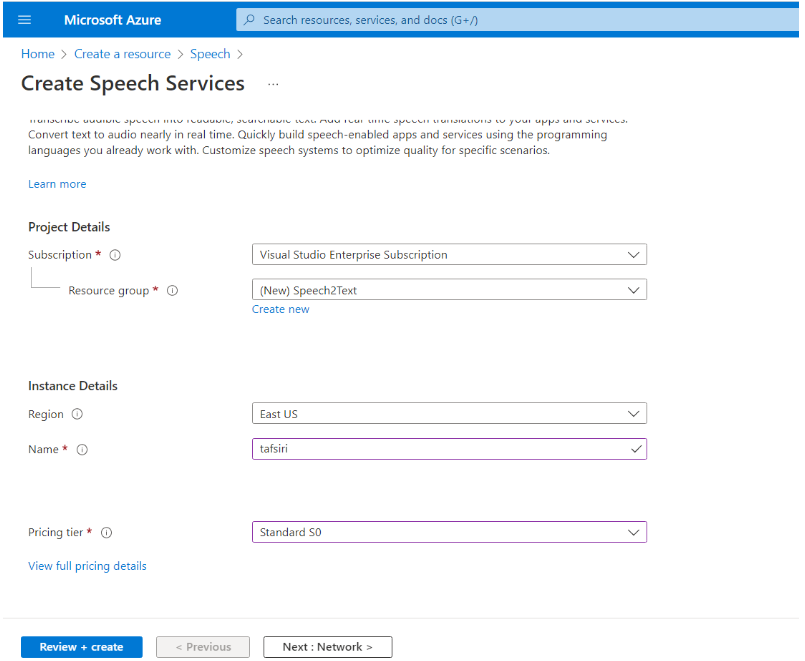
\includegraphics{./images/creating speech service.png}

\hypertarget{speech-to-text-api-call}{%
\section{Speech-to-text API call}\label{speech-to-text-api-call}}

Since now we have our audio sample input \texttt{sample.wav} ,we can now
go ahead to the transcribing bit. It is noteworthy that the speech to
text rest API for short audio has several limitations which are:

\begin{itemize}
\item
  Requests cannot contain more than 60 seconds of audio. For batch
  transcriptions and custom speech use
  \href{https://docs.microsoft.com/en-us/azure/cognitive-services/speech-service/rest-speech-to-text}{Speech
  to Text API v3.0}
\item
  The API does not provide partial results.
\item
  It does not support Speech translation. For translation, you can
  checkout the
  \href{https://docs.microsoft.com/en-us/azure/cognitive-services/speech-service/speech-sdk}{Speech
  SDK}
\end{itemize}

Now that we are done with that, we can then go ahead and get coding.

\textbf{\texttt{Note:}} To access the speech service we just created
from R, we need the \textbf{URL of the endpoint},
\textbf{location/region details} and \textbf{KEY 1 \& 2} parameters.
These can be found in the azure portal under \textbf{Keys and Endpoint}
page of your cognitive service resource as illustrated below:

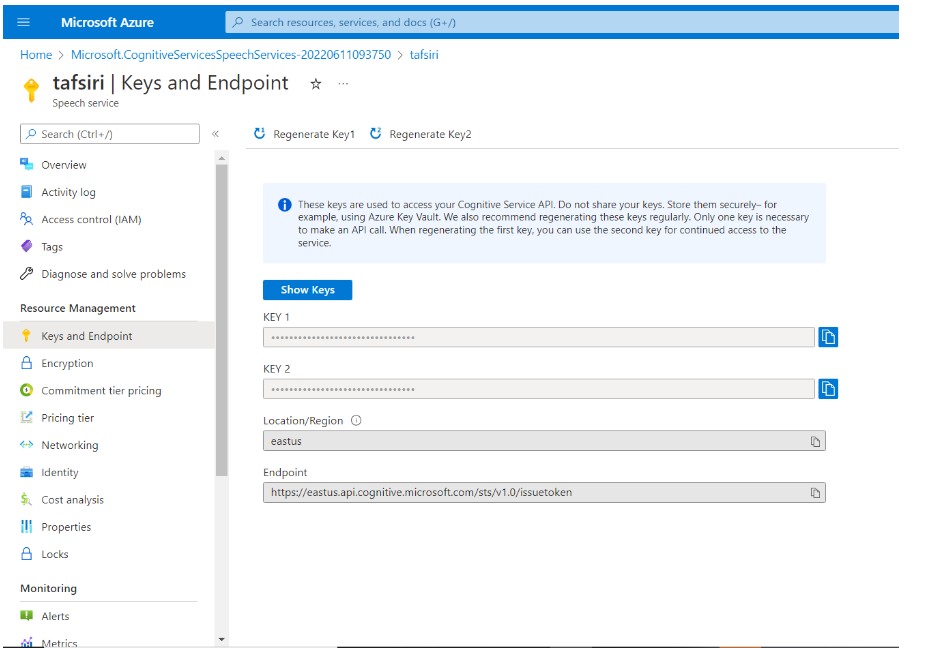
\includegraphics{./images/keys and endpoints.png}

Copy these details and save them since we are going to need them when
make our API call. Note: you can use either \textbf{KEY 1} or
\textbf{KEY 2} as your subscription key

To begin our transcription, install the packages we are going to need if
you don't have them already installed:

\begin{Shaded}
\begin{Highlighting}[]
\CommentTok{\#Enables us to work with HTTP in R}
\FunctionTok{install.packages}\NormalTok{(}\StringTok{"httr"}\NormalTok{) }
\FunctionTok{install.packages}\NormalTok{(}\StringTok{"jsonlite"}\NormalTok{)}
\end{Highlighting}
\end{Shaded}

\textbf{Note} You will have to modify the subscription key, language and
data path parameters to match the ones on the Cognitive Services
resource you created earlier. Also modify the URL
\texttt{\textquotesingle{}https://eastus.stt.speech.microsoft.com/speech/recognition/conversation/cognitiveservices/v1\textquotesingle{}}
by inserting the aforementioned location details as shown in the
modified URL :
\texttt{\textquotesingle{}https://\_ENTER\_LOCATION\_HERE\_.stt.speech.microsoft.com/speech/recognition/conversation/cognitiveservices/v1\textquotesingle{}}
. At the end you should have something like this:

\begin{Shaded}
\begin{Highlighting}[]
\FunctionTok{library}\NormalTok{(httr)}
\FunctionTok{library}\NormalTok{(jsonlite)  }
\CommentTok{\#Documentation on the two packages can be found by running ?httr and ?jsonlite commands respectively on the console.}

\CommentTok{\#Define headers containing subscription key and content type}
\NormalTok{headers }\OtherTok{=} \FunctionTok{c}\NormalTok{(}
  \StringTok{\textasciigrave{}}\AttributeTok{Ocp{-}Apim{-}Subscription{-}Key}\StringTok{\textasciigrave{}} \OtherTok{=} \StringTok{\textquotesingle{}\_ENTER\_YOUR\_SUBSCRIPTION\_KEY\_HERE\textquotesingle{}}\NormalTok{,  }\CommentTok{\#Key 1 or 2}
  \StringTok{\textasciigrave{}}\AttributeTok{Content{-}Type}\StringTok{\textasciigrave{}} \OtherTok{=} \StringTok{\textquotesingle{}audio/wav\textquotesingle{}} \CommentTok{\#Since we are transcribing a WAV file}
\NormalTok{)}

\CommentTok{\#Create a parameters list, in this case we specify the languange parameter}
\NormalTok{params }\OtherTok{=} \FunctionTok{list}\NormalTok{(}
  \StringTok{\textasciigrave{}}\AttributeTok{language}\StringTok{\textasciigrave{}} \OtherTok{=} \StringTok{\textquotesingle{}en{-}US\textquotesingle{}}
\NormalTok{)}

\CommentTok{\#Enter path to the audio file we just recorded and saved}
\NormalTok{data }\OtherTok{=} \FunctionTok{upload\_file}\NormalTok{ (}\StringTok{\textquotesingle{}Insert\_path\_to\_sample.wav\_here\textquotesingle{}}\NormalTok{) }

\CommentTok{\#Make the API call and save the response recived}
\NormalTok{response }\OtherTok{\textless{}{-}}\NormalTok{ httr}\SpecialCharTok{::}\FunctionTok{POST}\NormalTok{(}\AttributeTok{url =} \StringTok{\textquotesingle{}https://eastus.stt.speech.microsoft.com/speech/recognition/conversation/cognitiveservices/v1\textquotesingle{}}\NormalTok{, }
\NormalTok{httr}\SpecialCharTok{::}\FunctionTok{add\_headers}\NormalTok{(}\AttributeTok{.headers=}\NormalTok{headers), }\AttributeTok{query =}\NormalTok{ params, }\AttributeTok{body =}\NormalTok{ data)}

\CommentTok{\#Convert response received to a dataframe}
\NormalTok{result }\OtherTok{\textless{}{-}} \FunctionTok{fromJSON}\NormalTok{(}\FunctionTok{content}\NormalTok{(response, }\AttributeTok{as  =} \StringTok{\textquotesingle{}text\textquotesingle{}}\NormalTok{)) }
\NormalTok{txt\_output }\OtherTok{\textless{}{-}} \FunctionTok{as.data.frame}\NormalTok{(result)}

\CommentTok{\#Extract transcribed text}
\NormalTok{txt\_input }\OtherTok{\textless{}{-}}\NormalTok{ txt\_output[}\DecValTok{1}\NormalTok{,}\DecValTok{2}\NormalTok{]}
\NormalTok{txt\_input}
\end{Highlighting}
\end{Shaded}

And with that, we have successfully recorded audio and transcribed it
with the aid of Microsoft Azure Cognitive Services. The applications of
the cognitive services are wide and this is just but a glimpse of what
one can accomplish using the Speech to Text service. I'll leave it at
that. Thank you foR youR time. Cheers.

\bookmarksetup{startatroot}

\hypertarget{manipulator-kinematics}{%
\chapter{Manipulator kinematics}\label{manipulator-kinematics}}

Eric Wanjau and Ian Muchiri

\hfill\break

This Notebook illustrates how the manipulator will arrive at the desired
location as instructed by the speech input.

Kinematics is the science of motion that treats the subject without
regard to the forces that cause it.

\hypertarget{forward-kinematics}{%
\subsection{Forward Kinematics}\label{forward-kinematics}}

Forward kinematics addresses the problem of computing the
\textbf{position and orientation of the end effector} relative to the
user's workstation given the joint angles of the manipulator.

The forward kinematics were performed in accordance with the
\href{https://en.wikipedia.org/wiki/Denavit\%E2\%80\%93Hartenberg_parameters}{Denavit---Hartenberg
(D-H)} convention. According to the D-H convention, any robot can be
described kinematically by giving the values of four quantities,
typically known as the D-H parameters, for each link. The link length
\(a\) and the link twist \(\alpha\)quantities\emph{,} describe the link
itself and the remaining two; link offset \(d\) and the joint angle
\(\theta\) describe the link's connection to a neighboring link.

To perform the manipulator kinematics, link frames were attached to the
manipulator as shown in Figure~\ref{fig-dh}. In summary, link frames are
laid out as follows:

\begin{enumerate}
\def\labelenumi{\arabic{enumi}.}
\tightlist
\item
  The \(z-axis\) is in the direction of the joint axis.
\item
  The \(x-axis\) is parallel to the common normal.
\item
  The \(y-axis\) follows from the x-axis and z-axis by choosing it to be
  a right-handed coordinate system.
\end{enumerate}

\begin{figure}

\begin{minipage}[t]{0.50\linewidth}

{\centering 

\raisebox{-\height}{

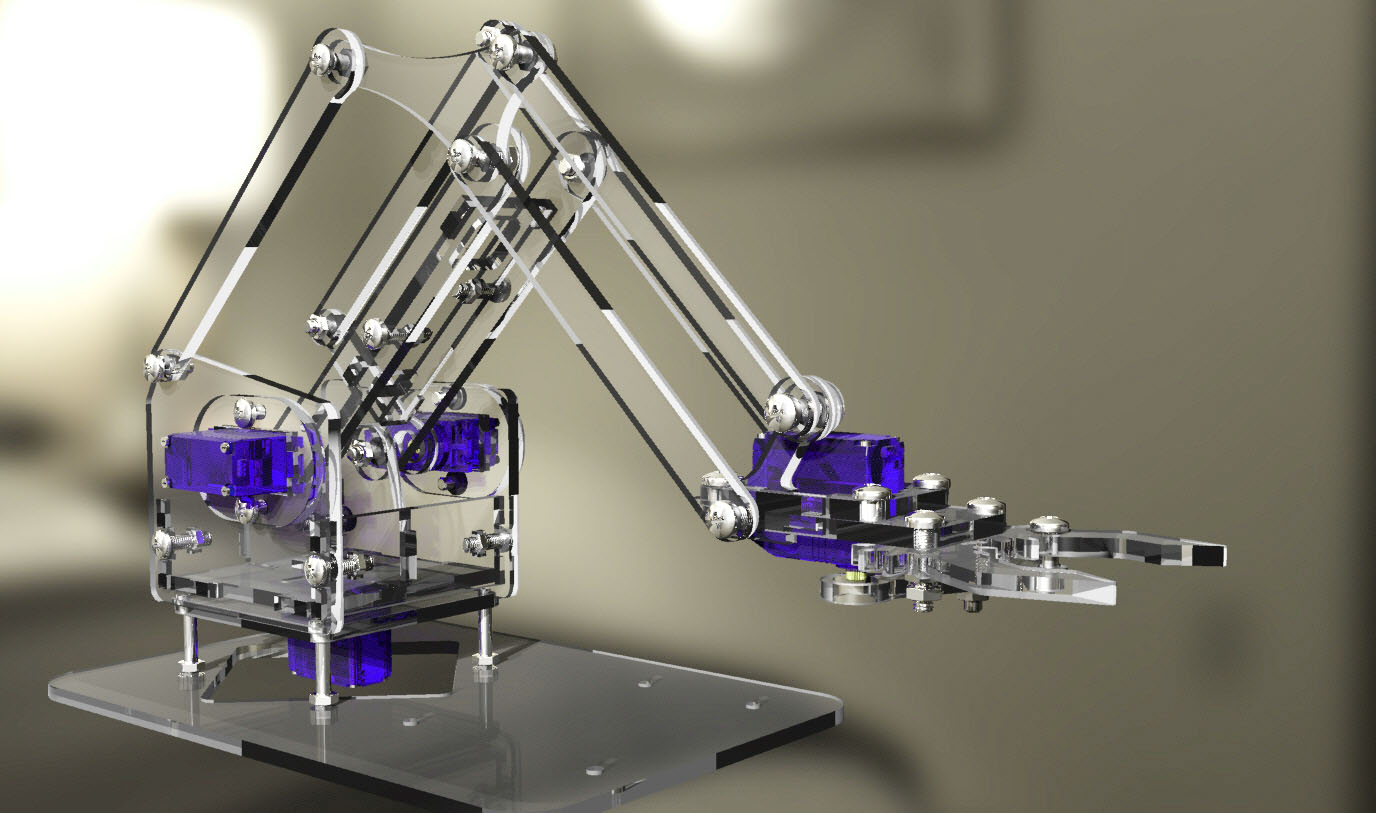
\includegraphics[width=4.16667in,height=\textheight]{./images/MeArm3D.jpg}

}

\caption{meArm parallel-link manipulator}

}

\end{minipage}%

\caption{\label{fig-dh}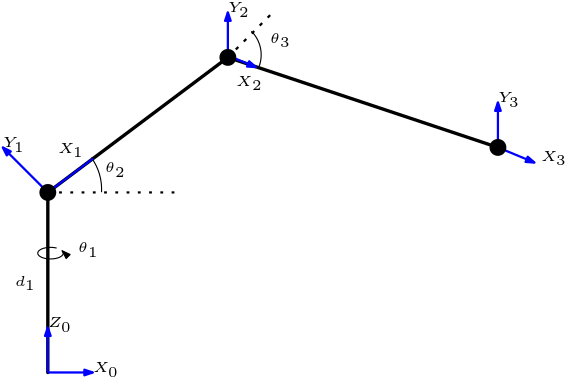
\includegraphics[width=4.16667in,height=\textheight]{./images/meArm.png}}

\end{figure}

Once the link frames have been laid, the D-H parameters can be easily
defined as:

\(d\): offset along the previous \(z\) to the common normal.

\(\theta\): angle about previous \(z\), from old \(x\) to new \(x\).

\(a\): length of the common normal.

\(\alpha\): angle about common normal from old \(z\ axis\) to new
\(z\ axis\).

The D-H parameters for the meArm were evaluated as below:

\begin{longtable}[]{@{}lllll@{}}
\caption{D-H parameters for meArm}\tabularnewline
\toprule()
Link & \(\theta\) & \(a(mm)\) & \(\alpha\) & \(d(mm)\) \\
\midrule()
\endfirsthead
\toprule()
Link & \(\theta\) & \(a(mm)\) & \(\alpha\) & \(d(mm)\) \\
\midrule()
\endhead
1 & \(\theta_1\) & 0 & 90 & 55 \\
2 & \(\theta_2\) & 80 & 0 & 0 \\
3 & \(\theta_3\) & 120 & 0 & 0 \\
\bottomrule()
\end{longtable}

In this convention, each homogeneous transformation \(A_i\) is
represented as a product of the four basic transformations (Spong,
Hutchinson, and Vidyasagar 2005), which evaluates to a \(4\times4\)
matrix that is used to transform a point from frame \(n\) to \(n\ -1\).

\[
A_i = Rot_{z, \theta_i}\ Trans_{x, a_i}\ Rot_{x, \alpha_i} \\
\]

\[
= \begin{bmatrix}
c_{\theta_i} & -s_{\theta_i} & 0 & 0 \\
s_{\theta_i} & c_{\theta_i} & 0 & 0 \\
0 & 0 & 1 & 0 \\
0 & 0 & 0 & 1
\end{bmatrix} 
\begin{bmatrix}
1 & 0 & 0 & 0 \\
0 & 1 & 0 & 0 \\
0 & 0 & 1 & d_i \\
0 & 0 & 0 & 1
\end{bmatrix}\\
\times \begin{bmatrix}
1 & 0 & 0 & a_i \\
0 & 1 & 0 & 0 \\
0 & 0 & 1 & 0 \\
0 & 0 & 0 & 1
\end{bmatrix}
\begin{bmatrix}
1 & 0 & 0 & 0 \\
0 & c_{\alpha_i} & -s_{\alpha_i} & 0 \\
0 & s_{\alpha_i} & c_{\alpha_i} & 0 \\
0 & 0 & 0 & 1
\end{bmatrix}
\]

\[
\begin{bmatrix}
c_{\theta_i} & -s_{\theta_i}c_{\alpha_i} & s_{\theta_i}c_{\alpha_i} & a_ic_{\theta_i} \\
s_{\theta_i} & c_{\theta_i}c_{\alpha_i} & -c_{\theta_i}s_{\alpha_i} & a_is_{\theta_i} \\
0 & s_{\alpha_i} & c_{\alpha_i} & d_i \\
0 & 0 & 0 & 1
\end{bmatrix}
\]

Considering the three links of the meArm, the total homogeneous
transformation will be a product of the transformations of the three
links given as:

\begin{equation}\protect\hypertarget{eq-transmat}{}{
A_T = A_1 \times A_2 \times A_3
}\label{eq-transmat}\end{equation}

The final total homogeneous transformation was derived to be:

\begin{equation}\protect\hypertarget{eq-totaltransmat}{}{
A_t =\ 
\begin{bmatrix}
cos(\theta_2 + \theta_3)cos(\theta_1) & -sin(\theta_2 + \theta_3)cos(\theta_1) & sin(\theta_1) & 4\sigma_1cos(\theta_1)
\\cos(\theta_2 + \theta_3)sin(\theta_1) & -sin(\theta_2 + \theta_3)sin(\theta_1) & -cos(\theta_1) & 4\sigma_1sin(\theta_1)
 \\
sin(\theta_2 + \theta_3) & cos(\theta_2 + \theta_3) & 0 & 12sin(\theta_2 + \theta_3) + 8sin(\theta_2) - \frac{11}{2}\\
0 & 0 & 0 & 1
\end{bmatrix}
}\label{eq-totaltransmat}\end{equation}

where

\[
\sigma_1 = 3\ cos(\theta_2 + \theta_3) + 2 \ cos(\theta_2)
\]

The position and orientation of the end effector \(x, y, z\) of the
meArm was consequently obtained from the total homogeneous
\(A_t\)transformation using the upper right 3x1 matrix as:

\begin{equation}\protect\hypertarget{eq-fkin}{}{
\begin{bmatrix}
x \\
y \\
z\end{bmatrix} = 
\begin{bmatrix}
4\cos(\theta_1) \ (3\ cos(\theta_2 + \theta_3) + 2 \ cos(\theta_2)) \\
4\sin(\theta_1) \ (3\ cos(\theta_2 + \theta_3) + 2 \ cos(\theta_2)) \\
12sin(\theta_2 + \theta_3) + 8sin(\theta_2) - \frac{11}{2}
\end{bmatrix}
}\label{eq-fkin}\end{equation}

\begin{tcolorbox}[enhanced jigsaw, colbacktitle=quarto-callout-tip-color!10!white, opacityback=0, breakable, bottomtitle=1mm, coltitle=black, arc=.35mm, left=2mm, titlerule=0mm, rightrule=.15mm, title=\textcolor{quarto-callout-tip-color}{\faLightbulb}\hspace{0.5em}{Tip}, colframe=quarto-callout-tip-color-frame, leftrule=.75mm, bottomrule=.15mm, toptitle=1mm, toprule=.15mm, opacitybacktitle=0.6, colback=white]
See
\href{https://github.com/R-icntay/research-papers/blob/main/papers/ENHANCING\%20PALLETIZING\%20AND\%20SHAPE\%20DRAWING\%20USING\%20IMAGE\%20PROCESSING\%20ON\%20PARALLEL\%20AND\%20SERIAL\%20LINK\%20MANIPULATORS(v7-Final).pdf}{this
paper} for a thorough derivation of the above.
\end{tcolorbox}

That said, let's put this into code:

\begin{Shaded}
\begin{Highlighting}[]
\CommentTok{\# Function that calculates forward kinematics}
\NormalTok{fkin }\OtherTok{\textless{}{-}} \ControlFlowTok{function}\NormalTok{(motor\_angles)\{}
  
  \CommentTok{\# Convert to radians}
\NormalTok{  angles }\OtherTok{=}\NormalTok{ motor\_angles }\SpecialCharTok{*}\NormalTok{ pi}\SpecialCharTok{/}\DecValTok{180}
  
  \CommentTok{\# Extract angles}
\NormalTok{  theta1 }\OtherTok{=}\NormalTok{ angles[}\DecValTok{1}\NormalTok{] }
\NormalTok{  theta2 }\OtherTok{=}\NormalTok{ angles[}\DecValTok{2}\NormalTok{]}
\NormalTok{  theta3 }\OtherTok{=}\NormalTok{ pi }\SpecialCharTok{{-}}\NormalTok{ angles[}\DecValTok{3}\NormalTok{]}
  
  \CommentTok{\# Calculate x, y, z}
\NormalTok{  x }\OtherTok{\textless{}{-}} \DecValTok{4} \SpecialCharTok{*} \FunctionTok{cos}\NormalTok{(theta1) }\SpecialCharTok{*}\NormalTok{( (}\DecValTok{3}\SpecialCharTok{*}\FunctionTok{cos}\NormalTok{(theta2 }\SpecialCharTok{+}\NormalTok{ theta3)) }\SpecialCharTok{+}\NormalTok{ (}\DecValTok{2}\SpecialCharTok{*}\FunctionTok{cos}\NormalTok{(theta2)))}
  
\NormalTok{  y }\OtherTok{\textless{}{-}} \DecValTok{4} \SpecialCharTok{*} \FunctionTok{sin}\NormalTok{(theta1) }\SpecialCharTok{*}\NormalTok{( (}\DecValTok{3}\SpecialCharTok{*}\FunctionTok{cos}\NormalTok{(theta2 }\SpecialCharTok{+}\NormalTok{ theta3)) }\SpecialCharTok{+}\NormalTok{ (}\DecValTok{2}\SpecialCharTok{*}\FunctionTok{cos}\NormalTok{(theta2)))}
  
\NormalTok{  z }\OtherTok{\textless{}{-}}\NormalTok{ (}\DecValTok{12} \SpecialCharTok{*} \FunctionTok{sin}\NormalTok{(theta2 }\SpecialCharTok{+}\NormalTok{ theta3)) }\SpecialCharTok{+}\NormalTok{ (}\DecValTok{8}\SpecialCharTok{*}\FunctionTok{sin}\NormalTok{(theta2)) }\SpecialCharTok{{-}}\NormalTok{ (}\DecValTok{11}\SpecialCharTok{/}\DecValTok{2}\NormalTok{)}
  
  
  \CommentTok{\# Return a tibble}
\NormalTok{  fkin }\OtherTok{\textless{}{-}} \FunctionTok{tibble}\NormalTok{(}
    
    \AttributeTok{orientation =} \FunctionTok{c}\NormalTok{(}\StringTok{"x"}\NormalTok{, }\StringTok{"y"}\NormalTok{, }\StringTok{"z"}\NormalTok{),}
    
    \CommentTok{\# Multiply by {-}1 to re{-}orient y and z}
    \CommentTok{\# mistake made during finding DH}
    
    \AttributeTok{position =} \FunctionTok{round}\NormalTok{(}\FunctionTok{c}\NormalTok{(x, y }\SpecialCharTok{*} \SpecialCharTok{{-}}\DecValTok{1}\NormalTok{, z }\SpecialCharTok{*} \SpecialCharTok{{-}}\DecValTok{1}\NormalTok{))}
    
\NormalTok{  )}
  
  \FunctionTok{return}\NormalTok{(fkin)}
  
  
  

\NormalTok{\}}
\end{Highlighting}
\end{Shaded}

What would be the \(x, y, z\) coordinates of the end effector when
rotation of motors \(1, 2, 3\) are \(90, 113, 78\) degrees respectively?

\begin{Shaded}
\begin{Highlighting}[]
\CommentTok{\# Calculate forward kinematics}
\FunctionTok{fkin}\NormalTok{(}\AttributeTok{motor\_angles =} \FunctionTok{c}\NormalTok{(}\DecValTok{90}\NormalTok{, }\DecValTok{113}\NormalTok{, }\DecValTok{78}\NormalTok{))}
\end{Highlighting}
\end{Shaded}

\begin{verbatim}
# A tibble: 3 x 2
  orientation position
  <chr>          <dbl>
1 x                  0
2 y                 13
3 z                  5
\end{verbatim}

\begin{Shaded}
\begin{Highlighting}[]
\FunctionTok{fkin}\NormalTok{(}\AttributeTok{motor\_angles =}\FunctionTok{c}\NormalTok{(}\DecValTok{42}\NormalTok{, }\DecValTok{110}\NormalTok{, }\DecValTok{114}\NormalTok{))}
\end{Highlighting}
\end{Shaded}

\begin{verbatim}
# A tibble: 3 x 2
  orientation position
  <chr>          <dbl>
1 x                -11
2 y                 10
3 z                 -3
\end{verbatim}

\hypertarget{inverse-kinematics}{%
\subsection{Inverse kinematics}\label{inverse-kinematics}}

Inverse kinematics addresses the more difficult converse problem of
computing the \textbf{set of joint angles} that will place the end
effector at a desired position and orientation. It is the computation of
the manipulator joint angles given the position and orientation of the
end effector.

In solving the inverse kinematics problem, the Geometric approach was
used to decompose the spatial geometry into several plane-geometry
problems based on the sine and the cosine rules. This was done by
considering the trigonometric decomposition of various planes of the
manipulator as graphically illustrated below:

\begin{figure}

\begin{minipage}[t]{0.50\linewidth}

{\centering 

\raisebox{-\height}{

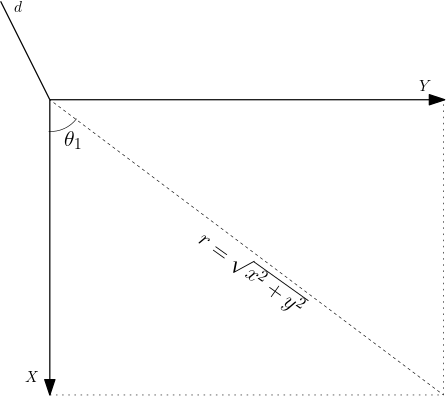
\includegraphics{./images/base_rotation.png}

}

}

\end{minipage}%
%
\begin{minipage}[t]{0.50\linewidth}

{\centering 

\raisebox{-\height}{

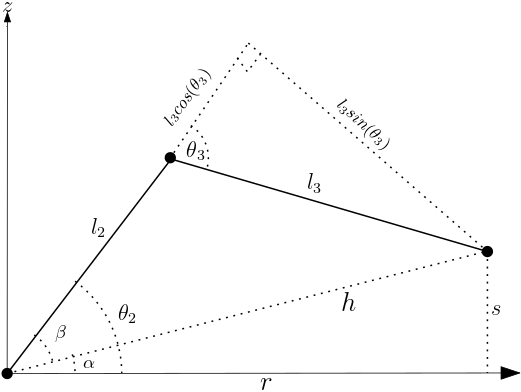
\includegraphics[width=4.64583in,height=\textheight]{./images/2nd_3rd.png}

}

}

\end{minipage}%

\end{figure}

\begin{equation}\protect\hypertarget{eq-theta1}{}{
\theta_1 = tan^{-1} \frac{y}{x}
}\label{eq-theta1}\end{equation}

With the hypotenuse r, connecting x and y obtained using the Pythagoras
theorem as

\[
r = \sqrt{x^2 + y^2}
\]

The angles \(\theta_2\) 𝑎𝑛𝑑 \(\theta_3\) were obtained by considering
the plane formed by the second and third links as illustrated:

\begin{equation}\protect\hypertarget{eq-theta2}{}{
\theta_2 = \alpha + \beta \\
\theta_2 = tan^{-1} \frac{s}{r} \ + tan^{-1} \frac{l_3sin(\theta_3)}{l_2 + l_3cos(\theta_3)}
}\label{eq-theta2}\end{equation}

\begin{equation}\protect\hypertarget{eq-theta3}{}{
\theta_3 = cos^{-1}\frac{x^2 + y^2 +s ^2 - l_2^2 - l_3^2}{2l_2l_3}
}\label{eq-theta3}\end{equation}

Where s is the difference between the distance of the end effector from
the base and the offset: \$\$ s = z- d

\$\$

Again, let's put the above into code

\begin{Shaded}
\begin{Highlighting}[]
\NormalTok{ikin }\OtherTok{\textless{}{-}} \ControlFlowTok{function}\NormalTok{(xyz\_coordinates)\{}
  
  \CommentTok{\# Extract xyz coordinates}
\NormalTok{  x }\OtherTok{=}\NormalTok{ xyz\_coordinates[}\DecValTok{1}\NormalTok{]}
\NormalTok{  y }\OtherTok{=}\NormalTok{ xyz\_coordinates[}\DecValTok{2}\NormalTok{]}
\NormalTok{  z }\OtherTok{=}\NormalTok{ xyz\_coordinates[}\DecValTok{3}\NormalTok{]}
  
  \CommentTok{\# Account for manipulator moving right or left}
  \ControlFlowTok{if}\NormalTok{ (x }\SpecialCharTok{\textgreater{}=} \DecValTok{0}\NormalTok{)\{}
\NormalTok{    theta1 }\OtherTok{=} \FunctionTok{atan}\NormalTok{(x}\SpecialCharTok{/}\NormalTok{y) }\SpecialCharTok{+}\NormalTok{ pi}\SpecialCharTok{/}\DecValTok{2}
\NormalTok{  \} }\ControlFlowTok{else}\NormalTok{ \{}
\NormalTok{    theta1 }\OtherTok{=} \FunctionTok{atan}\NormalTok{(y}\SpecialCharTok{/}\NormalTok{x) }\SpecialCharTok{\%\textgreater{}\%} \FunctionTok{abs}\NormalTok{()}
\NormalTok{  \}}
  
  \CommentTok{\# Calculate theta 3 since its needed in theta 2}
\NormalTok{  theta3 }\OtherTok{=} \FunctionTok{acos}\NormalTok{((x}\SpecialCharTok{\^{}}\DecValTok{2} \SpecialCharTok{+}\NormalTok{ y}\SpecialCharTok{\^{}}\DecValTok{2} \SpecialCharTok{+}\NormalTok{ (z}\DecValTok{{-}5}\NormalTok{)}\SpecialCharTok{\^{}}\DecValTok{2} \SpecialCharTok{{-}} \DecValTok{8}\SpecialCharTok{\^{}}\DecValTok{2} \SpecialCharTok{{-}} \DecValTok{12}\SpecialCharTok{\^{}}\DecValTok{2}\NormalTok{) }\SpecialCharTok{/}\NormalTok{ (}\DecValTok{2}\SpecialCharTok{*}\DecValTok{8}\SpecialCharTok{*}\DecValTok{12}\NormalTok{))}
    \CommentTok{\# 8 and 12 are the dimensions of manipulator arms}
  
  
  \CommentTok{\# Calculate theta 2}
\NormalTok{  theta2 }\OtherTok{=} \FunctionTok{atan}\NormalTok{((}\FloatTok{5.5} \SpecialCharTok{{-}}\NormalTok{ z) }\SpecialCharTok{/}\NormalTok{ (}\FunctionTok{sqrt}\NormalTok{(x}\SpecialCharTok{\^{}}\DecValTok{2} \SpecialCharTok{+}\NormalTok{ y}\SpecialCharTok{\^{}}\DecValTok{2}\NormalTok{)) ) }\SpecialCharTok{+} \FunctionTok{atan}\NormalTok{((}\DecValTok{12} \SpecialCharTok{*} \FunctionTok{sin}\NormalTok{(theta3)) }\SpecialCharTok{/}\NormalTok{ (}\DecValTok{8} \SpecialCharTok{+} \DecValTok{12}\SpecialCharTok{*}\FunctionTok{cos}\NormalTok{(theta3)))}
  
  \ControlFlowTok{if}\NormalTok{(theta2 }\SpecialCharTok{\textgreater{}} \DecValTok{0}\NormalTok{)\{}
\NormalTok{    theta2 }\OtherTok{=}\NormalTok{ pi }\SpecialCharTok{{-}} \FunctionTok{abs}\NormalTok{(theta2)}
\NormalTok{  \}}
  
\NormalTok{  tbl }\OtherTok{\textless{}{-}} \FunctionTok{tibble}\NormalTok{(}
    \AttributeTok{ef\_position =} \FunctionTok{c}\NormalTok{(x, y, z),}
    \AttributeTok{motor\_angles =}\NormalTok{ (}\FunctionTok{c}\NormalTok{(theta1, theta2, pi}\SpecialCharTok{{-}}\NormalTok{theta3)}\SpecialCharTok{*}\DecValTok{180}\SpecialCharTok{/}\NormalTok{pi) }\SpecialCharTok{\%\textgreater{}\%} \FunctionTok{round}\NormalTok{()}
\NormalTok{  )}
  
  \FunctionTok{return}\NormalTok{(tbl)}
  
\NormalTok{\}}
\end{Highlighting}
\end{Shaded}

Theoretically, the results from inverse kinematics and forward
kinematics should be in tandem for a given set of inputs. Let's see
whether we can get our previous joint angles from the results of the
forward kinematics.

\begin{Shaded}
\begin{Highlighting}[]
\CommentTok{\# Calculate inverse kinematics}
\FunctionTok{ikin}\NormalTok{(}\AttributeTok{xyz\_coordinates =} \FunctionTok{c}\NormalTok{(}\DecValTok{0}\NormalTok{, }\DecValTok{13}\NormalTok{, }\DecValTok{5}\NormalTok{))}
\end{Highlighting}
\end{Shaded}

\begin{verbatim}
# A tibble: 3 x 2
  ef_position motor_angles
        <dbl>        <dbl>
1           0           90
2          13          113
3           5           78
\end{verbatim}

\begin{Shaded}
\begin{Highlighting}[]
\FunctionTok{ikin}\NormalTok{(}\AttributeTok{xyz\_coordinates =} \FunctionTok{c}\NormalTok{(}\SpecialCharTok{{-}}\DecValTok{11}\NormalTok{, }\DecValTok{10}\NormalTok{, }\SpecialCharTok{{-}}\DecValTok{3}\NormalTok{))}
\end{Highlighting}
\end{Shaded}

\begin{verbatim}
# A tibble: 3 x 2
  ef_position motor_angles
        <dbl>        <dbl>
1         -11           42
2          10          110
3          -3          114
\end{verbatim}

\hypertarget{summary}{%
\section{Summary}\label{summary}}

From the above examples, the xyz coordinate values obtained from forward
kinematics operation produced the same input angles when passed through
the inverse kinematics equations. This will be essential for future
operations such as validating whether motor angle rotations result in a
desired xyz position of the end effector.

And with that, this section is done! Please do feel free to reach out in
case of any questions, feedback and suggestions.

Happy LeaRning,

\href{https://twitter.com/ericntay}{Eric}.

\bookmarksetup{startatroot}

\hypertarget{board-mapping}{%
\chapter{Board mapping}\label{board-mapping}}

Eric Wanjau and Ian Muchiri

\hfill\break

This notebook illustrates how we assigned real world board coordinates
(cm) to each square box on the chess board.

The approach was quite straightforward. We created a virtual board and
then translated virtual coordinates to the manipulator's workspace.

\begin{Shaded}
\begin{Highlighting}[]
\FunctionTok{library}\NormalTok{(here)}
\FunctionTok{library}\NormalTok{(waffle)}
\FunctionTok{library}\NormalTok{(patchwork)}
\FunctionTok{library}\NormalTok{(magick)}
\FunctionTok{library}\NormalTok{(tidyverse)}

\CommentTok{\# Vector}
\NormalTok{x }\OtherTok{\textless{}{-}} \FunctionTok{c}\NormalTok{(}\AttributeTok{A=} \DecValTok{1}\NormalTok{, }\AttributeTok{B =} \DecValTok{1}\NormalTok{, }\AttributeTok{C =} \DecValTok{1}\NormalTok{, }\AttributeTok{D =} \DecValTok{1}\NormalTok{, }\AttributeTok{E =} \DecValTok{1}\NormalTok{, }\AttributeTok{F =} \DecValTok{1}\NormalTok{, }\AttributeTok{G =} \DecValTok{1}\NormalTok{)}
\NormalTok{y }\OtherTok{\textless{}{-}} \FunctionTok{c}\NormalTok{(}\AttributeTok{A=} \DecValTok{1}\NormalTok{, }\AttributeTok{B =} \DecValTok{1}\NormalTok{, }\AttributeTok{C =} \DecValTok{1}\NormalTok{, }\AttributeTok{D =} \DecValTok{1}\NormalTok{, }\AttributeTok{E =} \DecValTok{1}\NormalTok{, }\AttributeTok{F =} \DecValTok{1}\NormalTok{, }\AttributeTok{G =} \DecValTok{1}\NormalTok{)}

\CommentTok{\# Create checker boxes}
\NormalTok{w1 }\OtherTok{=} \FunctionTok{waffle}\NormalTok{(x, }\AttributeTok{rows =} \DecValTok{8}\NormalTok{, }\AttributeTok{flip =} \ConstantTok{TRUE}\NormalTok{, }\AttributeTok{colors =} \FunctionTok{c}\NormalTok{(}\StringTok{"black"}\NormalTok{, }\StringTok{"white"}\NormalTok{, }\StringTok{"black"}\NormalTok{, }\StringTok{"white"}\NormalTok{, }\StringTok{"black"}\NormalTok{, }\StringTok{"white"}\NormalTok{, }\StringTok{"black"}\NormalTok{, }\StringTok{"white"}\NormalTok{), }\AttributeTok{legend\_pos =} \StringTok{""}\NormalTok{, , }\AttributeTok{size =} \FloatTok{0.1}\NormalTok{) }\SpecialCharTok{+} 
  \FunctionTok{theme}\NormalTok{(}\AttributeTok{plot.margin =} \FunctionTok{margin}\NormalTok{(}\DecValTok{0}\NormalTok{, }\DecValTok{0}\NormalTok{, }\DecValTok{0}\NormalTok{, }\DecValTok{0}\NormalTok{))}
\NormalTok{w2 }\OtherTok{=} \FunctionTok{waffle}\NormalTok{(y, }\AttributeTok{rows =} \DecValTok{8}\NormalTok{, }\AttributeTok{flip =} \ConstantTok{TRUE}\NormalTok{, }\AttributeTok{colors =} \FunctionTok{c}\NormalTok{(}\StringTok{"white"}\NormalTok{, }\StringTok{"black"}\NormalTok{, }\StringTok{"white"}\NormalTok{, }\StringTok{"black"}\NormalTok{, }\StringTok{"white"}\NormalTok{, }\StringTok{"black"}\NormalTok{, }\StringTok{"white"}\NormalTok{, }\StringTok{"black"}\NormalTok{), }\AttributeTok{legend\_pos =} \StringTok{""}\NormalTok{, }\AttributeTok{size =} \FloatTok{0.1}\NormalTok{) }\SpecialCharTok{+}
  \FunctionTok{theme}\NormalTok{(}\AttributeTok{plot.margin =} \FunctionTok{margin}\NormalTok{(}\DecValTok{0}\NormalTok{, }\DecValTok{0}\NormalTok{, }\DecValTok{0}\NormalTok{, }\DecValTok{0}\NormalTok{))}

\CommentTok{\# Make checker board}
\NormalTok{checkerboard }\OtherTok{\textless{}{-}}\NormalTok{ w1 }\SpecialCharTok{/}\NormalTok{ w2 }\SpecialCharTok{/}\NormalTok{ w1 }\SpecialCharTok{/}\NormalTok{ w2 }\SpecialCharTok{/}\NormalTok{ w1 }\SpecialCharTok{/}\NormalTok{ w2 }\SpecialCharTok{/}\NormalTok{ w1 }\SpecialCharTok{/}\NormalTok{ w2}
\NormalTok{checkerboard}
\end{Highlighting}
\end{Shaded}

\begin{figure}[H]

{\centering 
\includegraphics{./03_board_mapping_files/figure-pdf/unnamed-chunk-2-1.pdf}

}

\end{figure}

\begin{Shaded}
\begin{Highlighting}[]
\FunctionTok{ggsave}\NormalTok{(}\StringTok{"images/checkerboard.png"}\NormalTok{, }\AttributeTok{width =} \DecValTok{7}\NormalTok{, }\AttributeTok{height =} \DecValTok{7}\NormalTok{)}
\end{Highlighting}
\end{Shaded}

\hypertarget{convert-image-into-a-tibble}{%
\section{Convert image into a
tibble}\label{convert-image-into-a-tibble}}

\begin{Shaded}
\begin{Highlighting}[]
\FunctionTok{library}\NormalTok{(magick)}
\NormalTok{img }\OtherTok{\textless{}{-}} \FunctionTok{image\_read}\NormalTok{(}\StringTok{"images/checkerboard.png"}\NormalTok{) }\SpecialCharTok{\%\textgreater{}\%} 
  \FunctionTok{image\_convert}\NormalTok{(}\AttributeTok{type =} \StringTok{"grayscale"}\NormalTok{)}
\CommentTok{\# Dimensions of virtual board}
\NormalTok{dim\_x }\OtherTok{=} \DecValTok{160} \SpecialCharTok{*} \DecValTok{4}
\NormalTok{dim\_y }\OtherTok{=} \DecValTok{160} \SpecialCharTok{*} \DecValTok{4}
\NormalTok{img }\OtherTok{\textless{}{-}} \FunctionTok{image\_resize}\NormalTok{(img, }\FunctionTok{paste}\NormalTok{(dim\_x, dim\_y, }\AttributeTok{sep =} \StringTok{"x"}\NormalTok{))}


\CommentTok{\# Create row and column identifiers}
\NormalTok{row\_names }\OtherTok{\textless{}{-}}  \FunctionTok{tibble}\NormalTok{(}\AttributeTok{x =} \DecValTok{1}\SpecialCharTok{:}\NormalTok{dim\_x, }\AttributeTok{y =} \FunctionTok{rep}\NormalTok{(LETTERS[}\DecValTok{1}\SpecialCharTok{:}\DecValTok{8}\NormalTok{], }\AttributeTok{each =}\NormalTok{ dim\_y}\SpecialCharTok{/}\DecValTok{8}\NormalTok{), }\AttributeTok{z =} \FunctionTok{paste}\NormalTok{(x, }\StringTok{"\_"}\NormalTok{, y, }\AttributeTok{sep =} \StringTok{""}\NormalTok{)) }\SpecialCharTok{\%\textgreater{}\%} \FunctionTok{pull}\NormalTok{(z)}

\NormalTok{col\_names }\OtherTok{\textless{}{-}}  \FunctionTok{tibble}\NormalTok{(}\AttributeTok{x =} \DecValTok{1}\SpecialCharTok{:}\NormalTok{dim\_x, }\AttributeTok{y =} \FunctionTok{rep}\NormalTok{(}\DecValTok{1}\SpecialCharTok{:}\DecValTok{8}\NormalTok{, }\AttributeTok{each =}\NormalTok{ dim\_x}\SpecialCharTok{/}\DecValTok{8}\NormalTok{), }\AttributeTok{z =} \FunctionTok{paste}\NormalTok{(x, }\StringTok{"\_"}\NormalTok{, y, }\AttributeTok{sep =} \StringTok{""}\NormalTok{)) }\SpecialCharTok{\%\textgreater{}\%} \FunctionTok{pull}\NormalTok{(z)}

\CommentTok{\# Create array and number rows and columns}
\NormalTok{img\_array }\OtherTok{\textless{}{-}} \FunctionTok{drop}\NormalTok{(}\FunctionTok{as.integer}\NormalTok{(}\FunctionTok{pluck}\NormalTok{(img, }\DecValTok{1}\NormalTok{)))}
\FunctionTok{rownames}\NormalTok{(img\_array) }\OtherTok{\textless{}{-}}\NormalTok{ row\_names}
\FunctionTok{colnames}\NormalTok{(img\_array) }\OtherTok{\textless{}{-}}\NormalTok{ col\_names}


\CommentTok{\# Create data frame from array and rename column}
\NormalTok{img\_dfx }\OtherTok{\textless{}{-}}\NormalTok{ img\_array }\SpecialCharTok{\%\textgreater{}\%} 
  \FunctionTok{as\_tibble}\NormalTok{() }\SpecialCharTok{\%\textgreater{}\%} 
  \FunctionTok{mutate}\NormalTok{(}\AttributeTok{y =}\NormalTok{ row\_names) }\SpecialCharTok{\%\textgreater{}\%} 
  \CommentTok{\#rowid\_to\_column(var = "y") \%\textgreater{}\% }
  \FunctionTok{pivot\_longer}\NormalTok{(}\SpecialCharTok{!}\NormalTok{y, }\AttributeTok{names\_to =} \StringTok{"x"}\NormalTok{, }\AttributeTok{values\_to =} \StringTok{"pv"}\NormalTok{) }\SpecialCharTok{\%\textgreater{}\%} 
  \FunctionTok{mutate}\NormalTok{(}\AttributeTok{pv =}\NormalTok{ scales}\SpecialCharTok{::}\FunctionTok{rescale}\NormalTok{(pv, }\AttributeTok{to =} \FunctionTok{c}\NormalTok{(}\DecValTok{0}\NormalTok{, }\DecValTok{1}\NormalTok{))) }\SpecialCharTok{\%\textgreater{}\%} 
  \CommentTok{\# binarize image}
  \FunctionTok{mutate}\NormalTok{(}\AttributeTok{pv =} \FunctionTok{case\_when}\NormalTok{(}
\NormalTok{    pv }\SpecialCharTok{\textgreater{}} \FloatTok{0.5} \SpecialCharTok{\textasciitilde{}} \DecValTok{1}\NormalTok{,}
    \ConstantTok{TRUE} \SpecialCharTok{\textasciitilde{}} \DecValTok{0}\NormalTok{)) }\SpecialCharTok{\%\textgreater{}\%} 
  \FunctionTok{separate}\NormalTok{(y, }\FunctionTok{c}\NormalTok{(}\StringTok{"y"}\NormalTok{, }\StringTok{"pl"}\NormalTok{)) }\SpecialCharTok{\%\textgreater{}\%} 
  \FunctionTok{separate}\NormalTok{(x, }\FunctionTok{c}\NormalTok{(}\StringTok{"x"}\NormalTok{, }\StringTok{"pn"}\NormalTok{)) }\SpecialCharTok{\%\textgreater{}\%} 
  \FunctionTok{mutate}\NormalTok{(}\AttributeTok{pos =} \FunctionTok{paste}\NormalTok{(pl, pn, }\AttributeTok{sep =} \StringTok{""}\NormalTok{)) }\SpecialCharTok{\%\textgreater{}\%} 
  \FunctionTok{select}\NormalTok{(}\SpecialCharTok{{-}}\FunctionTok{c}\NormalTok{(pn, pl)) }\SpecialCharTok{\%\textgreater{}\%} 
  \FunctionTok{mutate}\NormalTok{(}\FunctionTok{across}\NormalTok{(}\FunctionTok{c}\NormalTok{(y, x, pv), as.numeric)) }\SpecialCharTok{\%\textgreater{}\%} 
  \FunctionTok{group\_by}\NormalTok{(pos) }\SpecialCharTok{\%\textgreater{}\%} 
  \FunctionTok{mutate}\NormalTok{(}\AttributeTok{centroidx =} \FunctionTok{round}\NormalTok{(}\FunctionTok{mean}\NormalTok{(x)), }\AttributeTok{centroidy =} \FunctionTok{round}\NormalTok{(}\FunctionTok{mean}\NormalTok{(y))) }\SpecialCharTok{\%\textgreater{}\%} 
  \FunctionTok{ungroup}\NormalTok{()}
\end{Highlighting}
\end{Shaded}

Only centroid locations are of importance. So we narrow down to that:

\begin{Shaded}
\begin{Highlighting}[]
\CommentTok{\# Obtain location centroids}
\NormalTok{centroids }\OtherTok{\textless{}{-}}\NormalTok{ img\_dfx }\SpecialCharTok{\%\textgreater{}\%} 
  \FunctionTok{ungroup}\NormalTok{() }\SpecialCharTok{\%\textgreater{}\%} 
  \FunctionTok{distinct}\NormalTok{(pos, centroidx, centroidy)}

\CommentTok{\# View centroids on the virtual board}
\NormalTok{centroids }\SpecialCharTok{\%\textgreater{}\%} 
  \FunctionTok{slice\_head}\NormalTok{(}\AttributeTok{n =} \DecValTok{10}\NormalTok{)}
\end{Highlighting}
\end{Shaded}

\begin{verbatim}
# A tibble: 10 x 3
   pos   centroidx centroidy
   <chr>     <dbl>     <dbl>
 1 A1           40        40
 2 A2          120        40
 3 A3          200        40
 4 A4          280        40
 5 A5          360        40
 6 A6          440        40
 7 A7          520        40
 8 A8          600        40
 9 B1           40       120
10 B2          120       120
\end{verbatim}

\hypertarget{mapping-coordinates-to-xy}{%
\section{Mapping coordinates to xy}\label{mapping-coordinates-to-xy}}

Once the centroid pixel coordinates were successfully extracted, the
next step involved translating them to their corresponding real-world
x-y coordinates in cm. This scaling from pixel values to cm values was
achieved by the mapping function or simply using
\texttt{scales::rescale()}:

\begin{Shaded}
\begin{Highlighting}[]
\CommentTok{\# Mapping function}
\NormalTok{map\_fun }\OtherTok{\textless{}{-}} \ControlFlowTok{function}\NormalTok{(value, from\_low, from\_high, to\_low, to\_high)\{}
  
\NormalTok{  mapped\_val }\OtherTok{=}\NormalTok{ (value }\SpecialCharTok{{-}}\NormalTok{ from\_low) }\SpecialCharTok{*}\NormalTok{ (to\_high }\SpecialCharTok{{-}}\NormalTok{ to\_low) }\SpecialCharTok{/}\NormalTok{ (from\_high }\SpecialCharTok{{-}}\NormalTok{ from\_low) }\SpecialCharTok{+}\NormalTok{ (to\_low)}
  
  \FunctionTok{return}\NormalTok{(mapped\_val)}
\NormalTok{\}}


\CommentTok{\# Map virtual board coordinates to manipulator workspace}
\NormalTok{centroids }\OtherTok{=}\NormalTok{ centroids }\SpecialCharTok{\%\textgreater{}\%} 
    \CommentTok{\# mutate(x\_mapped = map\_fun(centroidx, from\_low = 0, from\_high = dim\_x, to\_low = 9, to\_high = {-}9),}
    \CommentTok{\#        y\_mapped = map\_fun(centroidy, from\_low = 0, from\_high = 192, to\_low = 11, to\_high = 17)) \%\textgreater{}\% }
    
    \DocumentationTok{\#\# Using scales::rescale}
    \FunctionTok{mutate}\NormalTok{(}\AttributeTok{x\_mapped =}\NormalTok{ scales}\SpecialCharTok{::}\FunctionTok{rescale}\NormalTok{(centroidx, }\AttributeTok{to =} \FunctionTok{c}\NormalTok{(}\DecValTok{9}\NormalTok{, }\SpecialCharTok{{-}}\DecValTok{9}\NormalTok{), }\AttributeTok{from =} \FunctionTok{c}\NormalTok{(}\DecValTok{0}\NormalTok{, }\DecValTok{640}\NormalTok{)),}
           \AttributeTok{y\_mapped =}\NormalTok{ scales}\SpecialCharTok{::}\FunctionTok{rescale}\NormalTok{(centroidy, }\AttributeTok{to =} \FunctionTok{c}\NormalTok{(}\DecValTok{11}\NormalTok{, }\DecValTok{17}\NormalTok{), }\AttributeTok{from =} \FunctionTok{c}\NormalTok{(}\DecValTok{0}\NormalTok{, }\DecValTok{192}\NormalTok{))) }\SpecialCharTok{\%\textgreater{}\%} 
    \FunctionTok{mutate}\NormalTok{(}\FunctionTok{across}\NormalTok{(}\FunctionTok{where}\NormalTok{(is.numeric), round)) }\SpecialCharTok{\%\textgreater{}\%} 
    \CommentTok{\# Rearrange board positions to match our physical chess board}
    \FunctionTok{mutate}\NormalTok{(}
      \AttributeTok{pl =} \FunctionTok{rep}\NormalTok{(LETTERS[}\DecValTok{1}\SpecialCharTok{:}\DecValTok{8}\NormalTok{], }\AttributeTok{times =} \FunctionTok{nrow}\NormalTok{(centroids)}\SpecialCharTok{/}\DecValTok{8}\NormalTok{),}
      \AttributeTok{pn =} \FunctionTok{rep}\NormalTok{(}\DecValTok{1}\SpecialCharTok{:}\DecValTok{8}\NormalTok{, }\AttributeTok{each =} \FunctionTok{nrow}\NormalTok{(centroids)}\SpecialCharTok{/}\DecValTok{8}\NormalTok{),}
      \AttributeTok{pos =} \FunctionTok{paste}\NormalTok{(pl, pn, }\AttributeTok{sep =} \StringTok{""}\NormalTok{)) }\SpecialCharTok{\%\textgreater{}\%} 
    \FunctionTok{select}\NormalTok{(}\SpecialCharTok{{-}}\FunctionTok{c}\NormalTok{(pl, pn))}

\CommentTok{\# View centroids coordinates}
\NormalTok{centroids }\SpecialCharTok{\%\textgreater{}\%} 
  \FunctionTok{slice\_head}\NormalTok{(}\AttributeTok{n =} \DecValTok{10}\NormalTok{)}
\end{Highlighting}
\end{Shaded}

\begin{verbatim}
# A tibble: 10 x 5
   pos   centroidx centroidy x_mapped y_mapped
   <chr>     <dbl>     <dbl>    <dbl>    <dbl>
 1 A1           40        40        8       12
 2 B1          120        40        6       12
 3 C1          200        40        3       12
 4 D1          280        40        1       12
 5 E1          360        40       -1       12
 6 F1          440        40       -3       12
 7 G1          520        40       -6       12
 8 H1          600        40       -8       12
 9 A2           40       120        8       15
10 B2          120       120        6       15
\end{verbatim}

Now let's visualize our handy work:

\begin{Shaded}
\begin{Highlighting}[]
\FunctionTok{theme\_set}\NormalTok{(}\FunctionTok{theme\_void}\NormalTok{())}

\CommentTok{\# Create virtual board}
\NormalTok{centroids }\SpecialCharTok{\%\textgreater{}\%} 
  \FunctionTok{ggplot}\NormalTok{(}\AttributeTok{mapping =} \FunctionTok{aes}\NormalTok{(}\AttributeTok{x =}\NormalTok{ centroidx}\SpecialCharTok{*}\DecValTok{2}\NormalTok{, }\AttributeTok{y =}\NormalTok{ centroidy}\SpecialCharTok{*}\DecValTok{2}\NormalTok{)) }\SpecialCharTok{+}
  \FunctionTok{geom\_tile}\NormalTok{(}\FunctionTok{aes}\NormalTok{(}\AttributeTok{fill =} \FunctionTok{str\_extract}\NormalTok{(pos, }\StringTok{"[:alpha:]"}\NormalTok{)), }\AttributeTok{color =} \StringTok{"white"}\NormalTok{, }\AttributeTok{alpha =} \FloatTok{0.8}\NormalTok{, }\AttributeTok{size =} \FloatTok{0.8}\NormalTok{, }\AttributeTok{show.legend =} \ConstantTok{FALSE}\NormalTok{) }\SpecialCharTok{+}
  \FunctionTok{geom\_text}\NormalTok{(}\FunctionTok{aes}\NormalTok{(}\AttributeTok{x =}\NormalTok{ centroidx}\SpecialCharTok{*}\DecValTok{2}\NormalTok{, }\AttributeTok{y =}\NormalTok{ centroidy}\SpecialCharTok{*}\DecValTok{2} \SpecialCharTok{+} \DecValTok{2}\NormalTok{, }\AttributeTok{label =}\NormalTok{ pos), }\AttributeTok{color =} \StringTok{"black"}\NormalTok{, }\AttributeTok{size =} \FloatTok{3.5}\NormalTok{) }\SpecialCharTok{+}
  \FunctionTok{coord\_equal}\NormalTok{() }\SpecialCharTok{+}
  \CommentTok{\#paletteer::scale\_fill\_paletteer\_d("RColorBrewer::Set2") +}
  \FunctionTok{scale\_fill\_manual}\NormalTok{(}\AttributeTok{values =}\NormalTok{ paletteer}\SpecialCharTok{::}\FunctionTok{paletteer\_d}\NormalTok{(}\StringTok{"RColorBrewer::Set2"}\NormalTok{) }\SpecialCharTok{\%\textgreater{}\%} \FunctionTok{paste}\NormalTok{() }\SpecialCharTok{\%\textgreater{}\%} \FunctionTok{str\_replace}\NormalTok{(}\StringTok{"\#FFD92FFF"}\NormalTok{, }\StringTok{"\#FFC000FF"}\NormalTok{))}
\end{Highlighting}
\end{Shaded}

\begin{figure}[H]

{\centering 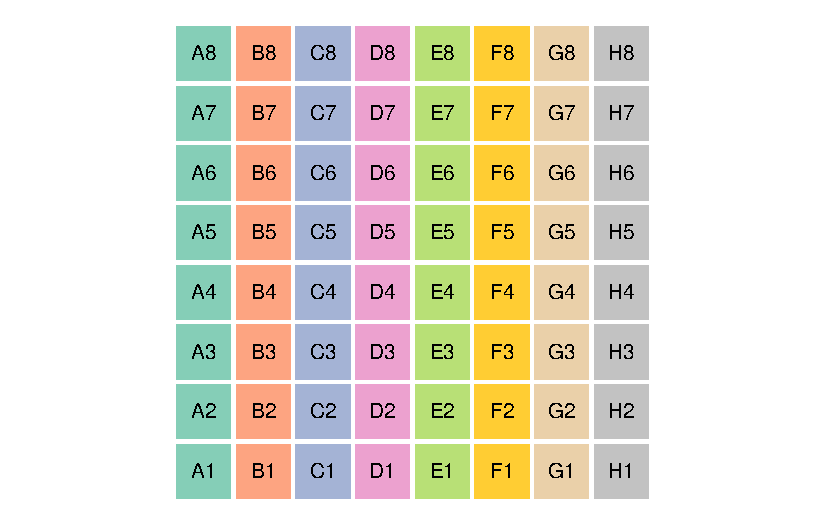
\includegraphics{./03_board_mapping_files/figure-pdf/unnamed-chunk-10-1.pdf}

}

\end{figure}

\begin{Shaded}
\begin{Highlighting}[]
\CommentTok{\# Virtual coordinates on board}
\NormalTok{centroids }\SpecialCharTok{\%\textgreater{}\%} 
  \FunctionTok{ggplot}\NormalTok{(}\AttributeTok{mapping =} \FunctionTok{aes}\NormalTok{(}\AttributeTok{x =}\NormalTok{ centroidx}\SpecialCharTok{*}\DecValTok{2}\NormalTok{, }\AttributeTok{y =}\NormalTok{ centroidy}\SpecialCharTok{*}\DecValTok{2}\NormalTok{)) }\SpecialCharTok{+}
  \FunctionTok{geom\_tile}\NormalTok{(}\FunctionTok{aes}\NormalTok{(}\AttributeTok{fill =} \FunctionTok{str\_extract}\NormalTok{(pos, }\StringTok{"[:alpha:]"}\NormalTok{)), }\AttributeTok{color =} \StringTok{"white"}\NormalTok{, }\AttributeTok{alpha =} \FloatTok{0.8}\NormalTok{, }\AttributeTok{size =} \FloatTok{0.8}\NormalTok{, }\AttributeTok{show.legend =} \ConstantTok{FALSE}\NormalTok{) }\SpecialCharTok{+}
  \FunctionTok{geom\_text}\NormalTok{(}\FunctionTok{aes}\NormalTok{(}\AttributeTok{x =}\NormalTok{ centroidx}\SpecialCharTok{*}\DecValTok{2}\NormalTok{, }\AttributeTok{y =}\NormalTok{ centroidy}\SpecialCharTok{*}\DecValTok{2} \SpecialCharTok{+} \DecValTok{2}\NormalTok{, }\AttributeTok{label =} \FunctionTok{paste}\NormalTok{(}\StringTok{"("}\NormalTok{, centroidx, }\StringTok{","}\NormalTok{, centroidy, }\StringTok{")"}\NormalTok{, }\AttributeTok{sep =} \StringTok{""}\NormalTok{)), }\AttributeTok{color =} \StringTok{"black"}\NormalTok{, }\AttributeTok{size =} \FloatTok{3.3}\NormalTok{) }\SpecialCharTok{+}
  \FunctionTok{coord\_equal}\NormalTok{() }\SpecialCharTok{+}
  \CommentTok{\#paletteer::scale\_fill\_paletteer\_d("RColorBrewer::Set2") +}
  \FunctionTok{scale\_fill\_manual}\NormalTok{(}\AttributeTok{values =}\NormalTok{ paletteer}\SpecialCharTok{::}\FunctionTok{paletteer\_d}\NormalTok{(}\StringTok{"RColorBrewer::Set2"}\NormalTok{) }\SpecialCharTok{\%\textgreater{}\%} \FunctionTok{paste}\NormalTok{() }\SpecialCharTok{\%\textgreater{}\%} \FunctionTok{str\_replace}\NormalTok{(}\StringTok{"\#FFD92FFF"}\NormalTok{, }\StringTok{"\#FFC000FF"}\NormalTok{))}
\end{Highlighting}
\end{Shaded}

\begin{figure}[H]

{\centering 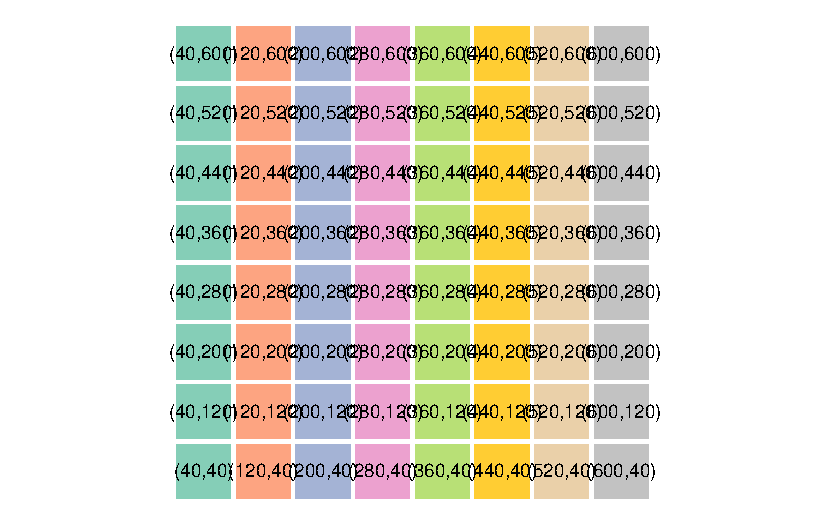
\includegraphics{./03_board_mapping_files/figure-pdf/unnamed-chunk-10-2.pdf}

}

\end{figure}

\begin{Shaded}
\begin{Highlighting}[]
\CommentTok{\# Real world coordinates on board}
\NormalTok{centroids }\SpecialCharTok{\%\textgreater{}\%} 
  \FunctionTok{ggplot}\NormalTok{(}\AttributeTok{mapping =} \FunctionTok{aes}\NormalTok{(}\AttributeTok{x =}\NormalTok{ centroidx}\SpecialCharTok{*}\DecValTok{2}\NormalTok{, }\AttributeTok{y =}\NormalTok{ centroidy}\SpecialCharTok{*}\DecValTok{2}\NormalTok{)) }\SpecialCharTok{+}
  \FunctionTok{geom\_tile}\NormalTok{(}\FunctionTok{aes}\NormalTok{(}\AttributeTok{fill =} \FunctionTok{str\_extract}\NormalTok{(pos, }\StringTok{"[:alpha:]"}\NormalTok{)), }\AttributeTok{color =} \StringTok{"white"}\NormalTok{, }\AttributeTok{alpha =} \FloatTok{0.8}\NormalTok{, }\AttributeTok{size =} \FloatTok{0.8}\NormalTok{, }\AttributeTok{show.legend =} \ConstantTok{FALSE}\NormalTok{) }\SpecialCharTok{+}
  \FunctionTok{geom\_text}\NormalTok{(}\FunctionTok{aes}\NormalTok{(}\AttributeTok{x =}\NormalTok{ centroidx}\SpecialCharTok{*}\DecValTok{2}\NormalTok{, }\AttributeTok{y =}\NormalTok{ centroidy}\SpecialCharTok{*}\DecValTok{2} \SpecialCharTok{+} \DecValTok{2}\NormalTok{, }\AttributeTok{label =} \FunctionTok{paste}\NormalTok{(}\StringTok{"("}\NormalTok{, x\_mapped, }\StringTok{","}\NormalTok{, y\_mapped, }\StringTok{")"}\NormalTok{, }\AttributeTok{sep =} \StringTok{""}\NormalTok{)), }\AttributeTok{color =} \StringTok{"black"}\NormalTok{, }\AttributeTok{size =} \FloatTok{3.3}\NormalTok{) }\SpecialCharTok{+}
  \FunctionTok{coord\_equal}\NormalTok{() }\SpecialCharTok{+}
  \CommentTok{\#paletteer::scale\_fill\_paletteer\_d("RColorBrewer::Set2") +}
  \FunctionTok{scale\_fill\_manual}\NormalTok{(}\AttributeTok{values =}\NormalTok{ paletteer}\SpecialCharTok{::}\FunctionTok{paletteer\_d}\NormalTok{(}\StringTok{"RColorBrewer::Set2"}\NormalTok{) }\SpecialCharTok{\%\textgreater{}\%} \FunctionTok{paste}\NormalTok{() }\SpecialCharTok{\%\textgreater{}\%} \FunctionTok{str\_replace}\NormalTok{(}\StringTok{"\#FFD92FFF"}\NormalTok{, }\StringTok{"\#FFC000FF"}\NormalTok{))}
\end{Highlighting}
\end{Shaded}

\begin{figure}[H]

{\centering 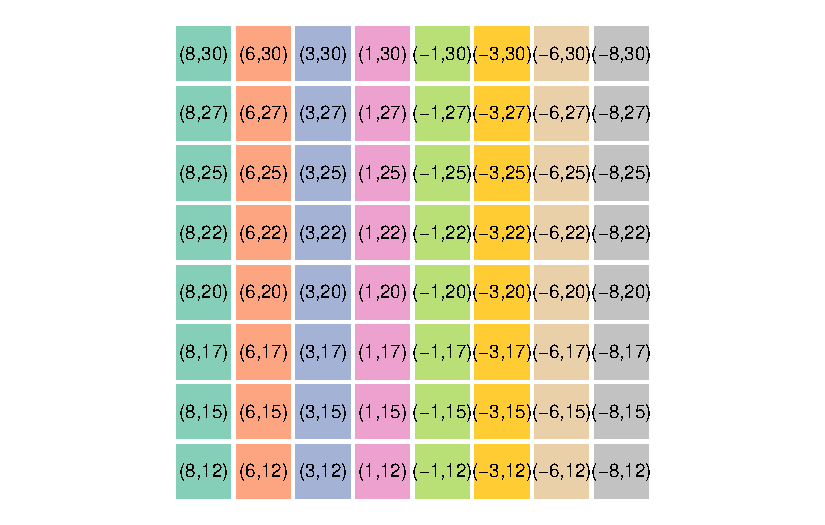
\includegraphics{./03_board_mapping_files/figure-pdf/unnamed-chunk-10-3.pdf}

}

\end{figure}

Here's an example of how we would extract the real word coordinates from
the tibble:

\begin{Shaded}
\begin{Highlighting}[]
\CommentTok{\# Function to return mapped values from tibble}
\NormalTok{get\_centroid }\OtherTok{\textless{}{-}} \ControlFlowTok{function}\NormalTok{(position)\{}
\NormalTok{  x }\OtherTok{=}\NormalTok{ centroids }\SpecialCharTok{\%\textgreater{}\%} 
    \FunctionTok{filter}\NormalTok{(}\FunctionTok{str\_detect}\NormalTok{(pos, position)) }\SpecialCharTok{\%\textgreater{}\%} 
    \FunctionTok{pull}\NormalTok{(x\_mapped)}
  
\NormalTok{  y }\OtherTok{=}\NormalTok{ centroids }\SpecialCharTok{\%\textgreater{}\%} 
    \FunctionTok{filter}\NormalTok{(}\FunctionTok{str\_detect}\NormalTok{(pos, position)) }\SpecialCharTok{\%\textgreater{}\%} 
    \FunctionTok{pull}\NormalTok{(y\_mapped)}
  
  \FunctionTok{return}\NormalTok{(}\FunctionTok{c}\NormalTok{(x, y))}
\NormalTok{\}}

\CommentTok{\# Define initial and final positions}
\NormalTok{initial\_pos }\OtherTok{\textless{}{-}} \StringTok{"B2"}
\NormalTok{final\_pos }\OtherTok{\textless{}{-}} \StringTok{"G2"}
\FunctionTok{get\_centroid}\NormalTok{(}\AttributeTok{position =}\NormalTok{ initial\_pos)}
\end{Highlighting}
\end{Shaded}

\begin{verbatim}
[1]  6 15
\end{verbatim}

\begin{Shaded}
\begin{Highlighting}[]
\FunctionTok{get\_centroid}\NormalTok{(}\AttributeTok{position =}\NormalTok{ final\_pos)}
\end{Highlighting}
\end{Shaded}

\begin{verbatim}
[1] -6 15
\end{verbatim}

\hypertarget{summary-1}{%
\section{Summary}\label{summary-1}}

This is the approach we took at this step. We created a virtual board
and then translated virtual coordinates to the manipulator's workspace.

And with that, this section is done! Please do feel free to reach out in
case of any questions, feedback and suggestions.

Happy Learning,

\href{https://twitter.com/ericntay}{Eric}.

\bookmarksetup{startatroot}

\hypertarget{r-and-arduino}{%
\chapter{R and Arduino}\label{r-and-arduino}}

Eric Wanjau and Ian Muchiri

\hfill\break

This notebook briefly describes how we set up a communication interface
between R and a microcontroller ( Arduino). Most of it is based on a
blog post we wrote a while back:
\href{https://rpubs.com/eR_ic/rduino}{\emph{What we R about when we R
about R and Arduino}}\textbf{\emph{.}}

\href{https://www.arduino.cc/en/Guide/Introduction}{\texttt{Arduino}} is
an open-source electronics platform based on easy-to-use hardware
(\texttt{Arduino\ Board}) and software (\texttt{Arduino\ IDE}). One can
tell the board what to do if one has the correct form of data and a set
of instructions for processing the data and performing subsequent
operations. The Arduino's microcontroller is responsible for holding all
your compiled code and executing the commands you specify. The Arduino
Software on the other hand is the board's IDE where one writes the set
of instructions governing the board. The getting
\href{https://www.arduino.cc/en/Guide}{started guide} would be a good
place to start learning about the Arduino ecosystem.

Switching over to R, we couldn't have found better words to summarize
what \texttt{R} is than with these words found in the book
\href{https://adv-r.hadley.nz/introduction.html}{Advanced R} by
\texttt{Hadley\ Wickham}: Despite its sometimes frustrating quirks, R
is, at its heart, an elegant and beautiful language, well tailored for
data science 🤗.

With all this said, a fine convergence can be struck between the two:
\texttt{data}. Consider this very simple example. We want the Arduino
board to turn an LED (Light Emitting Diode) ON once it receives a
\texttt{1} and OFF once it receives a \texttt{0}. If one can get a way
of sending some data (1 or 0) to the board's microcontroller, then, the
set objective will be achieved sooner or later.

\hypertarget{setting-up-a-serial-connection-between-r-and-arduino}{%
\subsection{Setting up a serial connection between R and
Arduino}\label{setting-up-a-serial-connection-between-r-and-arduino}}

Serial communication is the communication protocol that will be used
between R and the Arduino software similar to what is used in the
Arduino serial monitor. This communication interface will facilitate the
transmission of data between the two interfaces.

The serial package (Seilmayer 2020) will be used to set up this
comunication interface.

Let's begin by loading the required packages.

\begin{Shaded}
\begin{Highlighting}[]
\FunctionTok{library}\NormalTok{(tidyverse)}
\FunctionTok{library}\NormalTok{(serial)}
\FunctionTok{library}\NormalTok{(here)}
\end{Highlighting}
\end{Shaded}

Next, we'll create a serial port object called \texttt{arduino}, which
represents a serial client for communication with the USB serial port
where our board is connected.

\begin{Shaded}
\begin{Highlighting}[]
\CommentTok{\# See the ports available}
\FunctionTok{listPorts}\NormalTok{()}
\end{Highlighting}
\end{Shaded}

Create an Arduino object and set up the interface parameters.

This is achieved using the \texttt{serial::serialConnection} function.
The interface parameters are such that the baud rate (specifies the
number of bits being transferred per second) is set to \texttt{9600},
which is the same value in the Arduino script. Also, we have specified
that the transmission ends with a new line and that the transmission is
complete if the end of line symbol is the \texttt{carriage\ return\ cr}.

\begin{Shaded}
\begin{Highlighting}[]
\NormalTok{arduino }\OtherTok{\textless{}{-}}  \FunctionTok{serialConnection}\NormalTok{(}\AttributeTok{name =} \StringTok{"aRduino"}\NormalTok{,}
                           \AttributeTok{port =} \StringTok{"COM5"}\NormalTok{,}
                           \AttributeTok{mode =} \StringTok{"9600,n,8,1"}\NormalTok{ ,}
                           \AttributeTok{buffering =} \StringTok{"none"}\NormalTok{,}
                           \AttributeTok{newline =} \ConstantTok{TRUE}\NormalTok{,}
                           \AttributeTok{eof =} \StringTok{""}\NormalTok{,}
                           \AttributeTok{translation =} \StringTok{"cr"}\NormalTok{,}
                           \AttributeTok{handshake =} \StringTok{"none"}\NormalTok{,}
                           \AttributeTok{buffersize =} \DecValTok{8096}
                           
\NormalTok{                           )}
\end{Highlighting}
\end{Shaded}

Now that the serial interface is in place, the next step is initialising
the interface and keeping it open for later usage such as writing and
reading data from it. Once \texttt{serial::isOpen} initialises the
interface, the Arduino board blinks. This is because the board resets
once a serial port is opened to allow the bootloader to receive a new
sketch.

\texttt{serial::isOpen} tests whether the connection is open or not.

\begin{Shaded}
\begin{Highlighting}[]
\FunctionTok{open}\NormalTok{(arduino)}

\CommentTok{\# testing whether the connection is open or not}
\FunctionTok{isOpen}\NormalTok{(arduino)}
\end{Highlighting}
\end{Shaded}

\hypertarget{section}{%
\subsection{}\label{section}}

\hypertarget{writing-data-from-rstudio-to-the-serial-interface}{%
\subsection{\texorpdfstring{\textbf{Writing data from RStudio to the
serial
interface}}{Writing data from RStudio to the serial interface}}\label{writing-data-from-rstudio-to-the-serial-interface}}

At this point, we are all set to write some data to the serial
interface.

Let's prepare some data to send to the serial interface.

\begin{Shaded}
\begin{Highlighting}[]
\DocumentationTok{\#\# Create dummy data}
\NormalTok{n }\OtherTok{=} \DecValTok{42}
\NormalTok{arduino\_input }\OtherTok{\textless{}{-}} \FunctionTok{tibble}\NormalTok{(}
  \AttributeTok{c =} \FunctionTok{sample}\NormalTok{(}\DecValTok{10}\SpecialCharTok{:}\DecValTok{100}\NormalTok{, }\AttributeTok{size =}\NormalTok{ n, }\AttributeTok{replace =}\NormalTok{ T) }\SpecialCharTok{\%\textgreater{}\%}
                     \FunctionTok{paste}\NormalTok{(}\StringTok{\textquotesingle{}C\textquotesingle{}}\NormalTok{, }\AttributeTok{sep =} \StringTok{\textquotesingle{}\textquotesingle{}}\NormalTok{))}
\end{Highlighting}
\end{Shaded}

The chunk below uses \texttt{serial::write.serialConnection()} to write
the LED values to the serial port row by row.

\begin{Shaded}
\begin{Highlighting}[]
\FunctionTok{close}\NormalTok{(arduino)}
\FunctionTok{open}\NormalTok{(arduino)}
\FunctionTok{Sys.sleep}\NormalTok{(}\DecValTok{3}\NormalTok{)}
\ControlFlowTok{for}\NormalTok{ (r }\ControlFlowTok{in} \DecValTok{1}\SpecialCharTok{:}\FunctionTok{nrow}\NormalTok{(arduino\_input))\{}
  \FunctionTok{Sys.sleep}\NormalTok{(}\FloatTok{0.3}\NormalTok{)}
  \FunctionTok{write.serialConnection}\NormalTok{(arduino, }\FunctionTok{paste}\NormalTok{(arduino\_input[r,], }\AttributeTok{collapse =} \StringTok{\textquotesingle{}\textquotesingle{}}\NormalTok{))}
\NormalTok{\}}
\FunctionTok{Sys.sleep}\NormalTok{(}\DecValTok{2}\NormalTok{)}
\end{Highlighting}
\end{Shaded}

\hypertarget{driving-the-manipulators-servo-motors}{%
\subsection{Driving the manipulator's servo
motors}\label{driving-the-manipulators-servo-motors}}

The Arduino board itself is a programmable platform. You can tell your
board what to do by sending a set of instructions to the microcontroller
on the board. To do so you use the
\href{https://www.arduino.cc/en/Reference/HomePage}{Arduino programming
language} and \href{https://www.arduino.cc/en/Main/Software}{the Arduino
Software (IDE)}. Here are sample instructions that were uploaded to the
microcontroller:

\begin{Shaded}
\begin{Highlighting}[]

\ControlFlowTok{if}\OperatorTok{(}\NormalTok{Serial}\OperatorTok{.}\NormalTok{available}\OperatorTok{())\{} \CommentTok{// checks data in serial}

  \AttributeTok{static} \DataTypeTok{int}\NormalTok{ t}\OperatorTok{=}\DecValTok{0}\OperatorTok{;}

    \DataTypeTok{char}\NormalTok{ mychar}\OperatorTok{=}\NormalTok{Serial}\OperatorTok{.}\NormalTok{read}\OperatorTok{();} \CommentTok{// reads serial data}

    \ControlFlowTok{switch}\OperatorTok{(}\NormalTok{mychar}\OperatorTok{)\{}      

      \ControlFlowTok{case} \CharTok{\textquotesingle{}0\textquotesingle{}}\OperatorTok{...}\CharTok{\textquotesingle{}9\textquotesingle{}}\OperatorTok{:}

\NormalTok{        t}\OperatorTok{=}\NormalTok{t}\OperatorTok{*}\DecValTok{10} \OperatorTok{+}\NormalTok{ mychar }\OperatorTok{{-}} \CharTok{\textquotesingle{}0}\ErrorTok{’; // parse integers​}

        \ControlFlowTok{break}\OperatorTok{;}

      \ControlFlowTok{case} \CharTok{\textquotesingle{}A\textquotesingle{}}\OperatorTok{:}

        \OperatorTok{\{}

\NormalTok{            servoA}\OperatorTok{.}\NormalTok{write}\OperatorTok{(}\NormalTok{t}\OperatorTok{,}\DecValTok{50}\OperatorTok{,}\DecValTok{1}\OperatorTok{);} \CommentTok{// write value to motor}

\NormalTok{            Serial}\OperatorTok{.}\NormalTok{println}\OperatorTok{(}\NormalTok{t}\OperatorTok{);} \CommentTok{// print data to serial}

        \OperatorTok{\}}

\NormalTok{        t}\OperatorTok{=}\DecValTok{0}\OperatorTok{;}\NormalTok{​}

        \ControlFlowTok{break}\OperatorTok{;}\NormalTok{​}

        \OperatorTok{...}\NormalTok{​}

    \OperatorTok{\}}
\end{Highlighting}
\end{Shaded}

On a very high level, the microcontroller:

\begin{itemize}
\item
  Checks whether data is available on the serial interface.
\item
  Reads the data one byte at a time
\item
  Uses a series of switch case commands to

  \begin{itemize}
  \item
    Parse integers
  \item
    Write motor angles (send an electrical signal) to each respective
    motor based on the motor's tag e.g \texttt{A}, \texttt{B} or
    \texttt{C}
  \end{itemize}
\end{itemize}

So how do the servo motors actually rotate? Servos are controlled using
adjustable pulse widths on the signal line. This is achieved using a
technique called \texttt{Pulse\ Width\ Modulation}. PWM is a modulation
technique that generates variable-width pulses to represent the
amplitude of an analog input signal.

For a standard servo, sending a \texttt{1\ ms\ 5V} pulse turns the motor
to \texttt{0} degrees, and sending a \texttt{2\ ms\ 5V} pulse turns the
motor to \texttt{180} degrees, with pulse lengths in the middle scaling
linearly. A \texttt{1.5\ ms} pulse, for example, turns the motor to 90
degrees. Once a pulse has been sent, the servo turns to that position
and stays there until another pulse instruction is received. However, if
you want a servo to ``hold'' its position (resist being pushed on and
try to maintain the exact position), you just resend the command once
every 20 ms. The Arduino servo commands e.g \texttt{servo.write} takes
care of all this for you. To better understand how servo control works,
please see the timing diagram:

\begin{figure}

{\centering 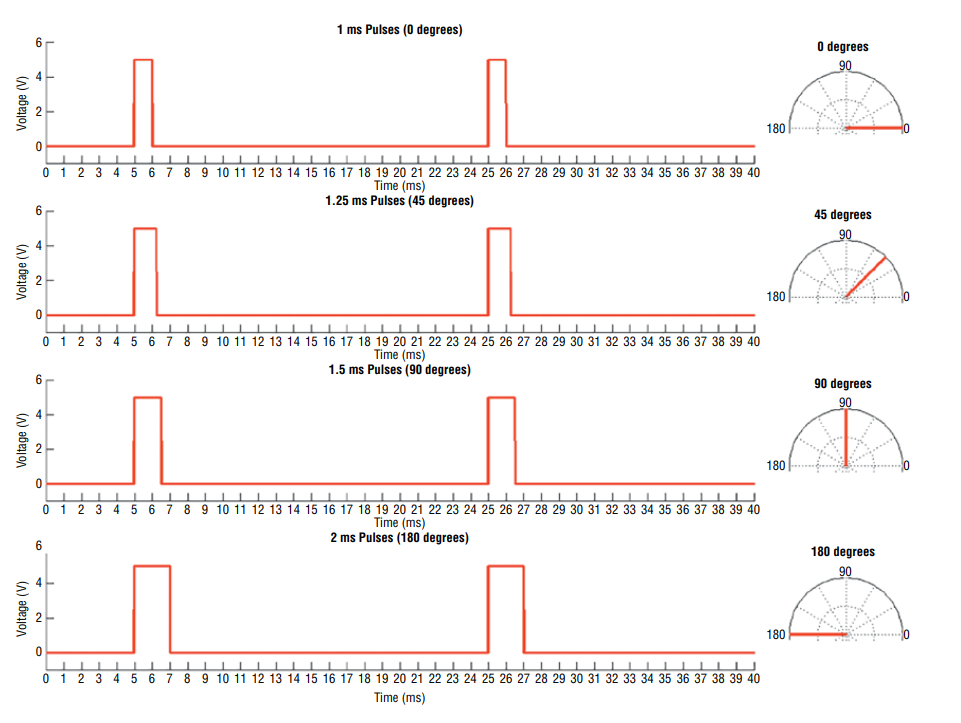
\includegraphics[width=5.20833in,height=\textheight]{./images/servo_timing.PNG}

}

\caption{Servo motor timing diagram: Jeremy Blum - Exploring Arduino}

\end{figure}

A great place to get started with Arduino and some hobby electronics
projects would be Blum (2013).

\hypertarget{reading-data-sent-from-arduino-board}{%
\subsection{\texorpdfstring{\textbf{Reading data sent from Arduino
board}}{Reading data sent from Arduino board}}\label{reading-data-sent-from-arduino-board}}

We can read the values sent to the serial port connection by Arduino
script using \texttt{read.serialConnection()}

\begin{Shaded}
\begin{Highlighting}[]
\NormalTok{data\_frm\_arduino }\OtherTok{\textless{}{-}} \FunctionTok{tibble}\NormalTok{(}\FunctionTok{capture.output}\NormalTok{(}\FunctionTok{cat}\NormalTok{(}\FunctionTok{read.serialConnection}\NormalTok{(arduino)))) }\SpecialCharTok{\%\textgreater{}\%} 
  \FunctionTok{filter}\NormalTok{(}\FunctionTok{if\_any}\NormalTok{(}\FunctionTok{where}\NormalTok{(is.character), }\SpecialCharTok{\textasciitilde{}}\NormalTok{ .x }\SpecialCharTok{!=} \StringTok{""}\NormalTok{))}


\NormalTok{data\_frm\_arduino}
\end{Highlighting}
\end{Shaded}

\hypertarget{summary-2}{%
\subsection{Summary}\label{summary-2}}

There we go! In this section, we leveraged Arduino's capability to be
programmed via a serial interface to send and receive data from R to the
Arduino board.

Please do feel free to reach out in case of any questions, feedback and
suggestions.

Happy Learning,

\href{https://twitter.com/ericntay}{Eric}.

\bookmarksetup{startatroot}

\hypertarget{summary-3}{%
\chapter{Summary}\label{summary-3}}

Awesome! That's how R played a role at each step of our project. You can
find how we combined the code chunks from these four chapters and the
user defined functions we created along the way to make our manipulator
move:
\href{https://github.com/R-icntay/rstudio_conf22_R_in_robotics/tree/main/R}{R}

The instructions on the microcontroller (described in chapter 4) that
send electrical pulses to rotate our motors can be found in the file
\href{https://github.com/R-icntay/rstudio_conf22_R_in_robotics/blob/main/arduino_code/robot_arm_control.ino}{robot\_arm\_control.ino}.

And that's it! There goes a touch of R in robotics.

Please do feel free to reach out in case of any questions, feedback and
suggestions,

\href{https://twitter.com/ericntay}{Eric} and
\href{https://twitter.com/Entity_4004}{Ian}.

\bookmarksetup{startatroot}

\hypertarget{references}{%
\chapter*{References}\label{references}}
\addcontentsline{toc}{chapter}{References}

\hypertarget{refs}{}
\begin{CSLReferences}{1}{0}
\leavevmode\vadjust pre{\hypertarget{ref-blum2013exploring}{}}%
Blum, J. 2013. \emph{Exploring Arduino: Tools and Techniques for
Engineering Wizardry}. EEET 2046 : Electronics. Wiley.
\url{https://books.google.co.uk/books?id=iXsQAAAAQBAJ}.

\leavevmode\vadjust pre{\hypertarget{ref-serial}{}}%
Seilmayer, Martin. 2020. {``Serial: The Serial Interface Package.''}
\url{https://CRAN.R-project.org/package=serial}.

\leavevmode\vadjust pre{\hypertarget{ref-spong2005robot}{}}%
Spong, M. W., S. Hutchinson, and M. Vidyasagar. 2005. \emph{Robot
Modeling and Control}. Wiley.

\end{CSLReferences}



\end{document}
